\documentclass[lettersize,journal]{IEEEtran}
\usepackage{amsmath,amsfonts}
\usepackage{algorithmic}
\usepackage{algorithm}
\usepackage{array}
\usepackage[caption=false,font=normalsize,labelfont=sf,textfont=sf]{subfig}
\usepackage{textcomp}
\usepackage{stfloats}
\usepackage{url}
\usepackage{verbatim}
\usepackage{graphicx}
\usepackage{cite}
%%%%%%%%%%%%%%%%%%%%%%%%%%%%%%%%%%%%%%%%%
% Journal Article
% LaTeX Template
% Version 1.4 (15/5/16)
%
% This template has been downloaded from:
% http://www.LaTeXTemplates.com
%
% Original author:
% Frits Wenneker (http://www.howtotex.com) with extensive modifications by
% Vel (vel@LaTeXTemplates.com)
%
% License:
% CC BY-NC-SA 3.0 (http://creativecommons.org/licenses/by-nc-sa/3.0/)
%
%%%%%%%%%%%%%%%%%%%%%%%%%%%%%%%%%%%%%%%%%

%----------------------------------------------------------------------------------------
%	PACKAGES AND OTHER DOCUMENT CONFIGURATIONS
%----------------------------------------------------------------------------------------

\usepackage{blindtext} % Package to generate dummy text throughout this template 

\usepackage[sc]{mathpazo} % Use the Palatino font
\usepackage[T1]{fontenc} % Use 8-bit encoding that has 256 glyphs
\linespread{1.05} % Line spacing - Palatino needs more space between lines
\usepackage{microtype} % Slightly tweak font spacing for aesthetics
\usepackage{float} % Force position of objects HERE

\usepackage[hang, small,labelfont=bf,up,textfont=it,up]{caption} % Custom captions under/above floats in tables or figures
\usepackage{booktabs} % Horizontal rules in tables
\usepackage{array}	% custom columns

\usepackage{lettrine} % The lettrine is the first enlarged letter at the beginning of the text

\usepackage{makecell}
\usepackage{enumitem} % Customized lists
\setlist[itemize]{noitemsep} % Make itemize lists more compact

\usepackage{abstract} % Allows abstract customization
\renewcommand{\abstractnamefont}{\normalfont\bfseries} % Set the "Abstract" text to bold
\renewcommand{\abstracttextfont}{\normalfont\small\itshape} % Set the abstract itself to small italic text

\usepackage{titlesec} % Allows customization of titles
\renewcommand\thesection{\Roman{section}} % Roman numerals for the sections
\renewcommand\thesubsection{\roman{subsection}} % roman numerals for subsections
\titleformat{\section}[block]{\large\scshape\centering}{\thesection.}{1em}{} % Change the look of the section titles
\titleformat{\subsection}[block]{\large}{\thesubsection.}{1em}{} % Change the look of the section titles

\usepackage{fancyhdr} % Headers and footers
%\pagestyle{fancy} % All pages have headers and footers
%\fancyfoot[RO,LE]{\thepage} % Custom footer text

\usepackage{titling} % Customizing the title section

\usepackage{hyperref} % For hyperlinks in the PDF
\usepackage{IEEEtrantools}
 \usepackage{mathtools}
\usepackage{amssymb} 

\usepackage{amsmath}
\usepackage{graphicx}
\usepackage{xfrac}
\usepackage{subcaption}
\usepackage{physics}

\usepackage{tikz}
\usepackage{environ}
\usepackage[export]{adjustbox}

\usepackage{csquotes}
\usepackage{multirow}
\usepackage{siunitx}
\sisetup{uncertainty-mode = separate}
\usepackage{isotope}
\usetikzlibrary{positioning,fit,calc}
\tikzset{block/.style={draw,thick,text width=2cm,minimum height=1cm,align=center},
	line/.style={-latex}
}

\makeatletter
\newsavebox{\measure@tikzpicture}
\NewEnviron{scaletikzpicturetowidth}[1]{%
  \def\tikz@width{#1}%
  \def\tikzscale{1}\begin{lrbox}{\measure@tikzpicture}%
  \BODY
  \end{lrbox}%
  \pgfmathparse{#1/\wd\measure@tikzpicture}%
  \edef\tikzscale{\pgfmathresult}%
  \BODY
}
\makeatother

%----------------------------------------------------------------------------------------
%	TITLE SECTION
%----------------------------------------------------------------------------------------

\setlength{\droptitle}{-4\baselineskip} % Move the title up

\pretitle{\begin{center}\Huge\bfseries} % Article title formatting
\posttitle{\end{center}} % Article title closing formatting

%================================================================================
%	MATHEMATICAL ABBREVIATIONS
%================================================================================
\renewcommand{\inf}{\infty}		% infinity
\newcommand{\I}{{i\mkern1mu}}	% sqrt(-1)
\newcommand{\ee}{\mathrm{e}}	% euler constant
\renewcommand{\exp}[1]{\mathrm{e}^{\left\{#1\right\}}}	% exponential function
\newcommand{\wt}[1]{\widetilde{#1}}
\newcommand{\ft}{\widetilde{\phi}}	% wide til phi
\newcommand{\qed}{\hfill\blacksquare}
\newcommand{\pdt}[1][]{\partial_{t}^{#1}}		% partial time derivative
\newcommand{\pdx}[1][]{\partial_{x}^{#1}}		% partial time derivative

%\newcommand{\el}{\mathrm{e^{-}}		% electron
%\newcommand{\ep}{\mathrm{e^{+}}}		% positron
%================================================================================
%	PLASMA ABBREVIATIONS
%================================================================================
\newcommand{\qT}{q_{_{T}}}			% test charge
\newcommand{\qs}{q_{_{s}}}			% species charge
\newcommand{\qo}{q_{_{0}}}			% charge
\newcommand{\vvo}{\vb{v}_{_0}}			% species velocity
\newcommand{\vvs}{\vb{v}_{_s}}			% species velocity
\newcommand{\vve}{\vb{v}_{_e}}			% electron velocity
\newcommand{\vvi}{\vb{v}_{_i}}			% ion velocity
\newcommand{\no}{n_{_{0}}}			% density
\newcommand{\ns}[1][]{n_{_{s#1}}}	% density: species [order]
\renewcommand{\ne}[1][]{n_{_{e#1}}}	% density: electron [order]
\renewcommand{\ni}[1][]{n_{_{i#1}}}	% density: ion [order]
\newcommand{\Ts}{T_{_{s}}}			% temperature: species
\newcommand{\Te}{T_{_{e}}}			% temperature: electron
\newcommand{\Ti}{T_{_{i}}}			% temperature: ion 
\newcommand{\ms}{m_{_{s}}}			% mass: species 
\newcommand{\me}{m_{_{e}}}			% mass: electron 
\newcommand{\mi}{m_{_{i}}}			% mass: ion
\newcommand{\evac}{\epsilon_{_{0}}}	% vacuum permeability
\newcommand{\lD}[1][]{\lambda_{_{D{#1}}}}	% [species] Debye's length
\newcommand{\kB}{k_{_B}}					% Boltzmann's constant
\newcommand{\dB}[1][]{\frac{e\phi}{\kB T_{_{#1}}}}	% Boltzmann distribution
%================================================================================
%	QUANTUM MECHANICS ABBREVIATIONS
%================================================================================
\newcommand{\ac}{a^{\dagger}}			% creation operator
\newcommand{\sa}{\ket{\alpha}}			% state 
\newcommand{\sacc}{\bra{\alpha}}			% state complex conjugate
\newcommand{\cO}{\mathcal{O}}			% Order

%\csname endofdump\endcsname

\usepackage[english]{babel} % Language hyphenation and typographical rules
\usepackage{derivative}		% derivative  

\newcommand{\pmseparator}{\hspace{0.2mm}\ensuremath{\pm}\hspace{0.2mm}}
\newcolumntype{+}{@{\pmseparator}}
%\endofdump
\usepackage[shell]{gnuplottex}
\hyphenation{op-tical net-works semi-conduc-tor IEEE-Xplore}
% updated with editorial comments 8/9/2021

\begin{document}

\title{Laboratorial Work nº1 - Proximity detector}

\author{João Guilherme 105939, Pedro Silva 107322, Martim Pinto 106290\\
\thanks{Group 4A - L02. This report is for the General Electronics class, 2024/2025.}}

% The paper headers
\markboth{Laboratorial report for General Electronics class 2024/2025, Group 4A}%
{Guilherme \MakeLowercase{\textit{et al.}}: Laboratorial Work nº1 - Proximity detector}

\maketitle

\begin{abstract}
This work focuses on designing a proximity detector using an infrared (IR) emitter and phototransistor to measure obstacle distance. The signal is processed through a rectifier, filter, and displayed using LEDs. Key achievements include assembling the circuit and validating its operation through simulation and experiments, while difficulties arose in aligning theoretical and experimental results.
\end{abstract}

\begin{IEEEkeywords} Proximity detector, infrared emitter, phototransistor, rectifier, bandpass filter, LED indicator, distance measurement, circuit design. 
\end{IEEEkeywords}

\section{Introduction}
\IEEEPARstart{T}{his} project focuses on designing a proximity detector, commonly used in applications such as automotive parking aids and industrial automation, for non-contact distance measurement. The system utilizes an infrared (IR) emitter and phototransistor, with the reflected signal processed through filtering and rectification, and the distance displayed using LEDs. The goal is to develop a functional circuit while gaining practical experience in design, simulation, and testing.

\section{Rectifier with filtering}
\subsection{Theoretical analysis}

The circuit in figure \ref{fig:circuit_components} can be divided into three main components:
\begin{itemize}
    \item A: High pass filter
    \item B: Voltage follower
    \item C: Peak detector (rectifier)
\end{itemize}

We will start by analysing the component A by determining it's transfer function:

\begin{equation}
    \label{eq:high_pass_1}
    T(s) = \frac{V_1}{V_{BP}} = \frac{Z_R}{Z_R + Z_C} = \frac{R_1sC_1}{1 + R_1sC_1}
\end{equation}

This transfer function corresponds to a high pass filter, having a zero at $s = 0$ and a pole at $s = -\frac{1}{R_1C_1}$. The transfer function starts with a positive slope of $20$ dB/Decade until it reaches the pole, corresponding to a cutoff frequency of $\omega_c = \frac{1}{R_1C_1}$ (rad/s).\\

To make sure that there exists a pole at $\approx$ 10 rad/s, the following relation must hold: $\frac{1}{R_1C_1} = 10$. Solving for $C_1$ and considering $R_1 = \SI{100}{\kilo \ohm}$ the result is \SI{1}{\micro \farad}.\\

\begin{figure}
    \centering
    \resizebox{\linewidth}{!}{
        \begin{gnuplot}[terminal=cairolatex, scale=1]

set logscale x

# Set labels for axes
set xlabel "Frequency (rad/s)"
set ylabel "Gain (dB)"
set y2label "Phase (degrees)"

# Set the range for the x-axis (x values)
set xrange [1:10000]

# Configure y-tics for both left and right axes
set ytics nomirror
set y2tics

# Define the constants
R = 100 * 10**3
C = 1 * 10**-6

# Define the functions
f(x) = 20*log10(x * R * C / (1 + x * R * C))
phi(x) = 90 - atan(x * R * C) * (180 / pi)

# Plot the functions
plot f(x) title "20 * log₁₀|T(s)|" with lines lw 2, \
     phi(x) title "Phase" with lines dashtype 2 lw 2 axes x1y2

\end{gnuplot}

    }
    \caption{Bode plot of the transfer function from the high-pass filter (component A).}
    \label{graph:transfer_function_1}
\end{figure}

Considering $T(s)$ for a square wave with \SI{5}{\volt} amplitude, \SI{2.5}{\volt} DC offset and $f = \SI{1}{\kilo \hertz}$ we obtain $|T(2\pi j \times f)| \approx 0.998$. To simplify further calculations, we will consider this value to be $1$, so the amplitude of the signal will not change. The filter will remove the DC ($f = \SI{0}{\hertz}$) component completely. The output signal should be in phase with the input signal.

The value of $v_1$ is then expected to be:

\begin{equation}
    v_1(t) = 2.5 \times \text{square}(\SI{1}{\kilo \hertz}) \quad \text{(V)}
    \label{eq:signal_v1}
\end{equation}

In theory, an ideal op-amp has infinite input impedance, meaning no current flows into the input terminals. However, in practice, this is not the case. Real op-amps have input bias currents — a small but non-zero amount of current that flows into the input terminals of the op-amp. These bias currents can lead to additional voltages that are undesirable in circuits, propagating errors to the output voltage. When large resistors are used, the input bias currents get higher, as less current goes trough the higher resistance. Therefore $R_1$ should be much lower than the op-amp’s input resistance.

The component B is performing as a buffer, isolating the low impedance component C from the high impedance of component A, it's acting as a voltage follower. The value of $v_2$ should match (in an ideal case, with ideal components) the value of $v_1$ (eq. \ref{eq:signal_v1}), assuming the op-amp does not saturate ($-12 \leq v_1 \leq 12$).\\ 

The component C is working as a peak detector. The diode D1 rectifies the signal allowing only the part of the signal with a value greater than the threshold voltage of $\SI{0.6}{\volt}$ to pass. The capacitor $C_2$ and the resistor $R_2$ are smoothing out the signal, converting an alternating signal into an almost constant DC signal. The output has a voltage corresponding to the peak value of the alternating input signal minus the threshold voltage.

\begin{equation}
    v_{dist} (t) = 2.5 - 0.6 = 1.9 \quad \text{(V)}
    \label{eq:vdist_signal}
\end{equation}

To verify computationally the theoretical results, we simulated the circuit using the software LTSpice. The software has a minor flaw where it defaults the rise/fall time of the square wave to $5\%$ of the period, even when set to 0, which causes the voltage values to not match the theoretical expectations. To fix this issue, we need to set the rise/fall time to \SI{1}{\us} in order to achieve a nearly 'perfect' square wave. The complete parameters used for the simulation can be found in appendix \ref{fig:ltspice_sim_settings_week1}.

\begin{figure}
    \centering
    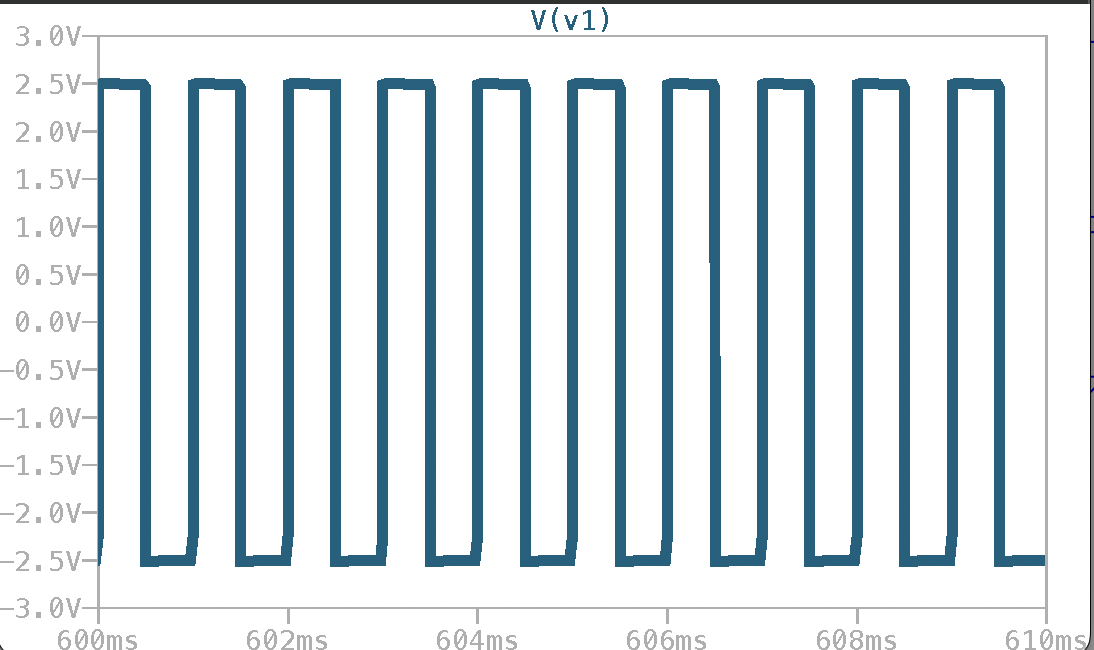
\includegraphics[width=\linewidth]{images/week1_v1.png}
    \caption{Graph of the voltage at node v1 simulated using LTSpice.}
    \label{fig:v_1-sim}
\end{figure}

\begin{figure}
    \centering
    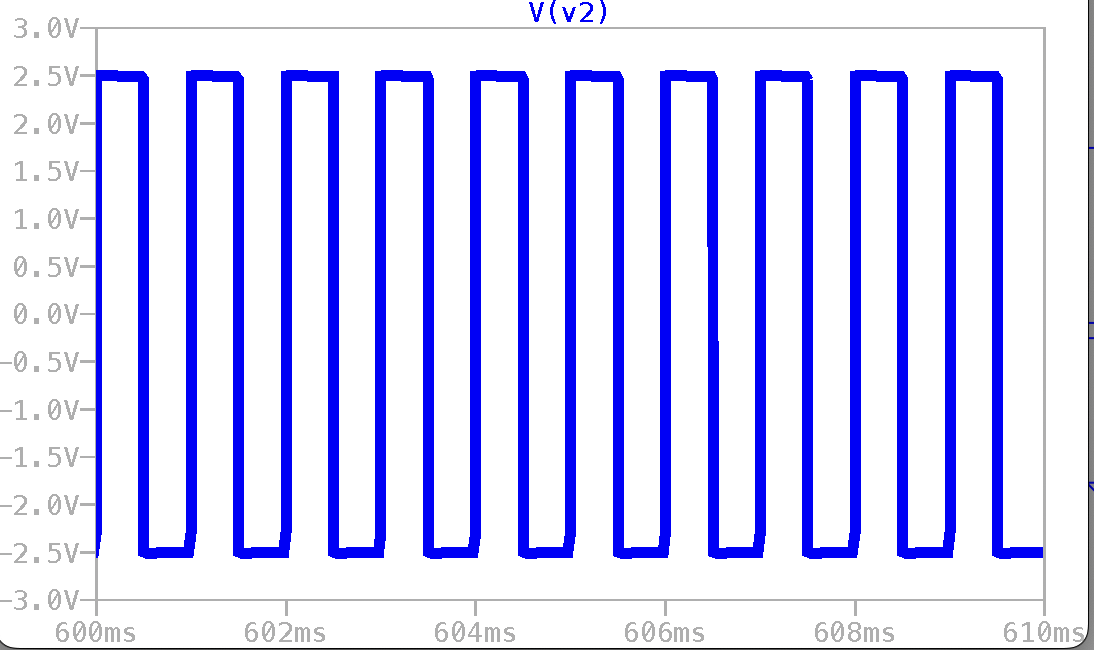
\includegraphics[width=\linewidth]{images/week1_v2.png}
    \caption{Graph of the voltage at node v2 simulated using LTSpice.}
    \label{fig:v2-sim}
\end{figure}

Both figures \ref{fig:v_1-sim} and \ref{fig:v2-sim} align with the theoretical expectation derived in equation \ref{eq:signal_v1}.

\begin{figure}
    \centering
    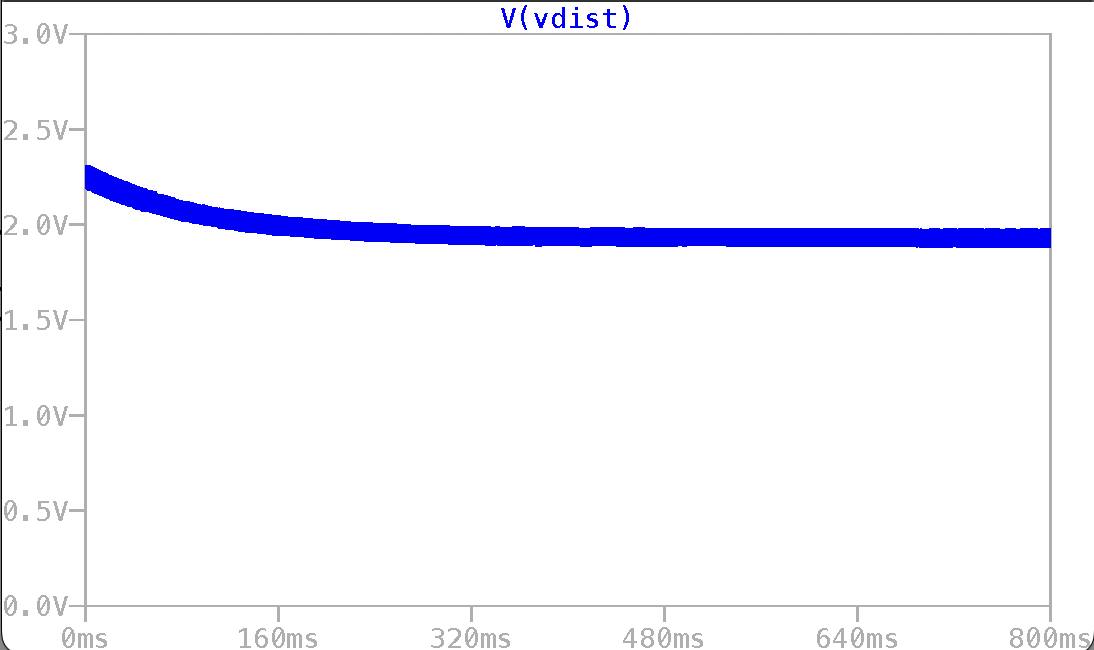
\includegraphics[width=\linewidth]{images/week1_vdist.png}
    \caption{Graph of the voltage at node vdist simulated using LTSpice.}
    \label{fig:vdist-sim}
\end{figure}

After a transient period that lasts about \SI{300}{\ms}, where the capacitors are still charging, the value of $v_{dist}$ converges to about $\SI{1.9}{\volt}$, which agrees with the derived value from equation \ref{eq:vdist_signal}.

\subsection{Experimental results}

As expected in the theoretical analysis (eq. \ref{eq:signal_v1}), the high pass filter should remove the DC component and maintain the amplitude of the signal, as the cutoff frequency is much lower than $\SI{1}{\kilo \hertz}$.\\

The observed signal in the oscilloscope (fig. \ref{fig:v1}) is aligned with the theoretical prediction, being centered around \SI{0}{V} (DC component removed) and with an amplitude peak-to-peak of \SI{5.225}{\volt} (the input signal from the wave generator has an amplitude greater than \SI{5}{\volt}).

\begin{figure}
    \centering
    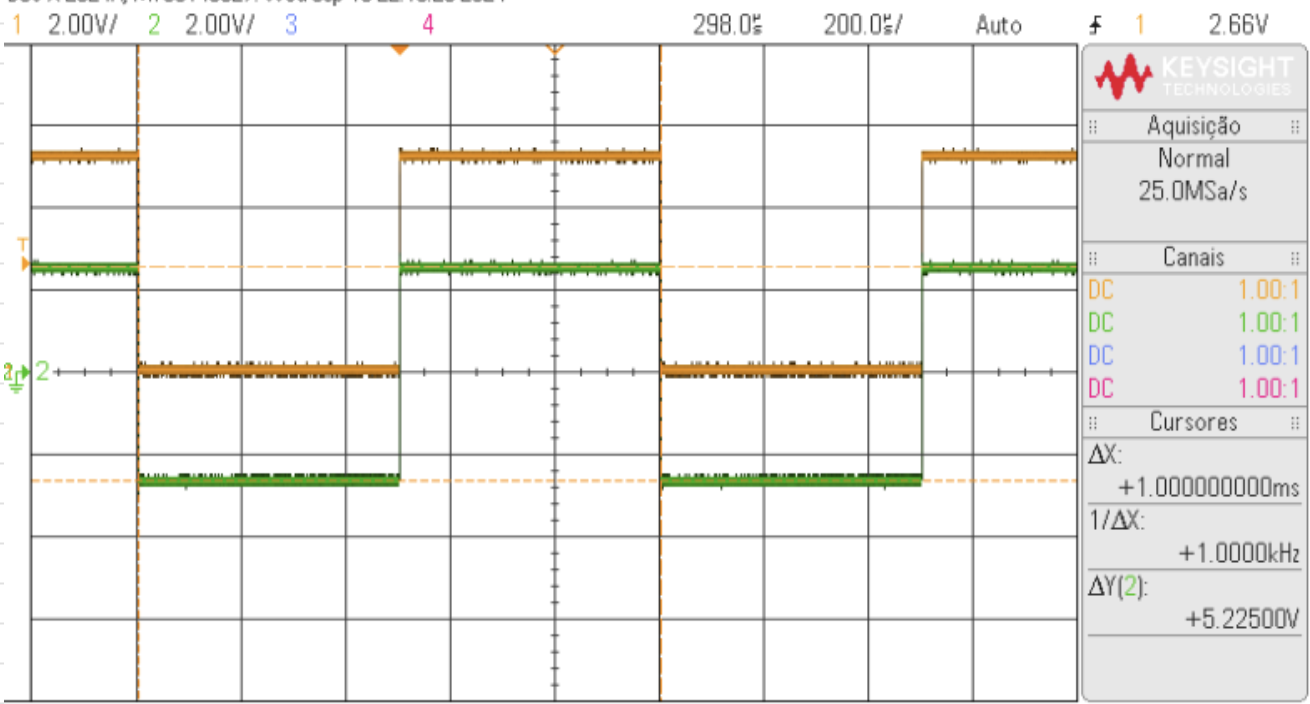
\includegraphics[width=\linewidth]{images/v1_scope.png}
    \caption{Observed $v_1$ signal (measured after the high pass filter) from the oscilloscope. The input signal is on channel 1.}
    \label{fig:v1}
\end{figure}

The signal then goes through the voltage follower (fig. \ref{fig:v2}), the output signal did not change in amplitude, which agrees with the theoretical prediction. There is a slight change of the shape of the signal in the ascent/descent, and that is due to the op-amp's imperfections, specifically, the slew-rate limitation. It is possible to calculate the slew-rate by dividing the voltage difference by the time it takes to reach it. The calculated slew-rate is \SI{0.42 \pm 0.09}{\volt / \us}, which agrees with the tabulated slew-rate of $\SI{0.5}{\volt / \us}$ in Texas Instruments's 741 IC amp-op datasheet.\\

We experimented modifying the load resistance after the voltage follower and verified that there where no significant changes between $v_1$ and $v_2$, therefore we can conclude that the op-amp is working as expected, isolating the high impedance source from the low impedance load, preventing the impact of the signal at $v_2$. 

\begin{figure}
    \centering
    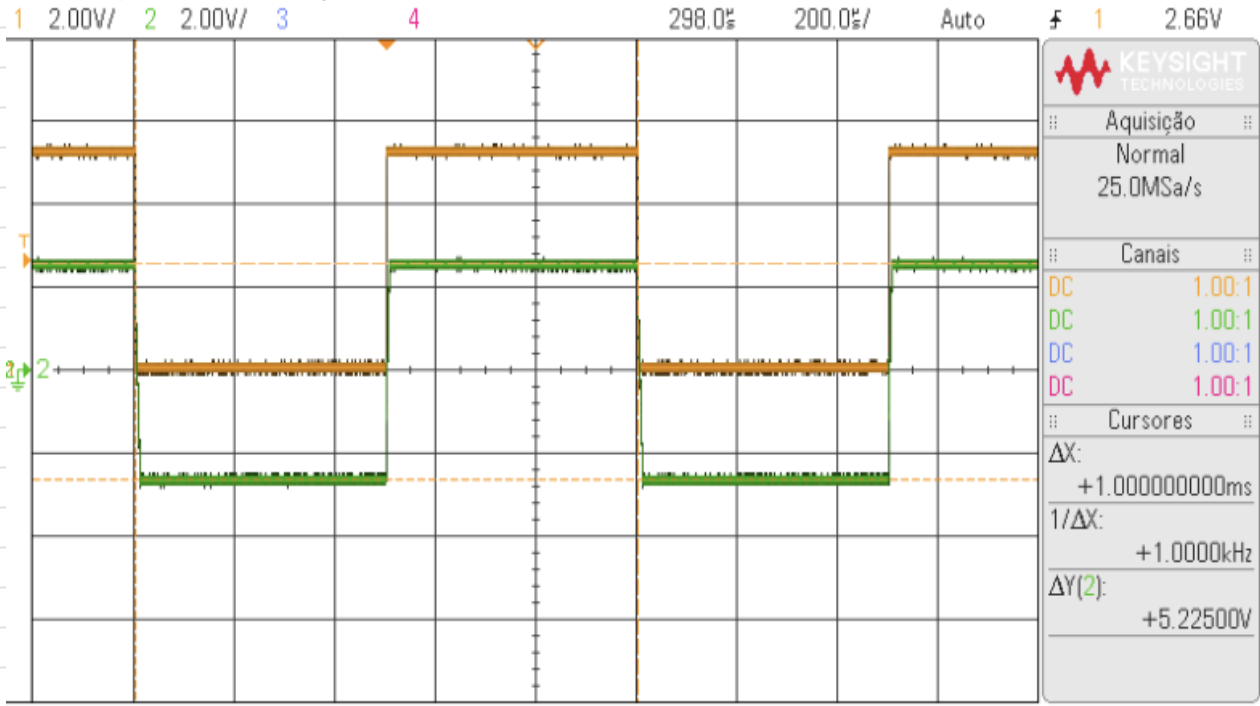
\includegraphics[width=\linewidth]{images/v2_scope.png}
    \caption{Observed $v_2$ signal (measured after the voltage follower) from the oscilloscope. The input signal is on channel 1.}
    \label{fig:v2}
\end{figure}
\vspace{20pt}

Finally, as the signal \( v_{\text{dist}} \) in fig. \ref{fig:vdist} remains almost constant, we successfully rectified and smoothed the previous \( v_2 \) signal, just as we anticipated. It is worth noting the low variation of \SI{125}{\m \volt} in the value of $v_{dist}$. The measured $v_{dist}$ value is \SI{1.938 \pm 0.063}{\volt}, which is in range with the predicted value of \SI{1.9}{\volt} from eq. \ref{eq:vdist_signal}. 

\begin{figure}
    \centering
    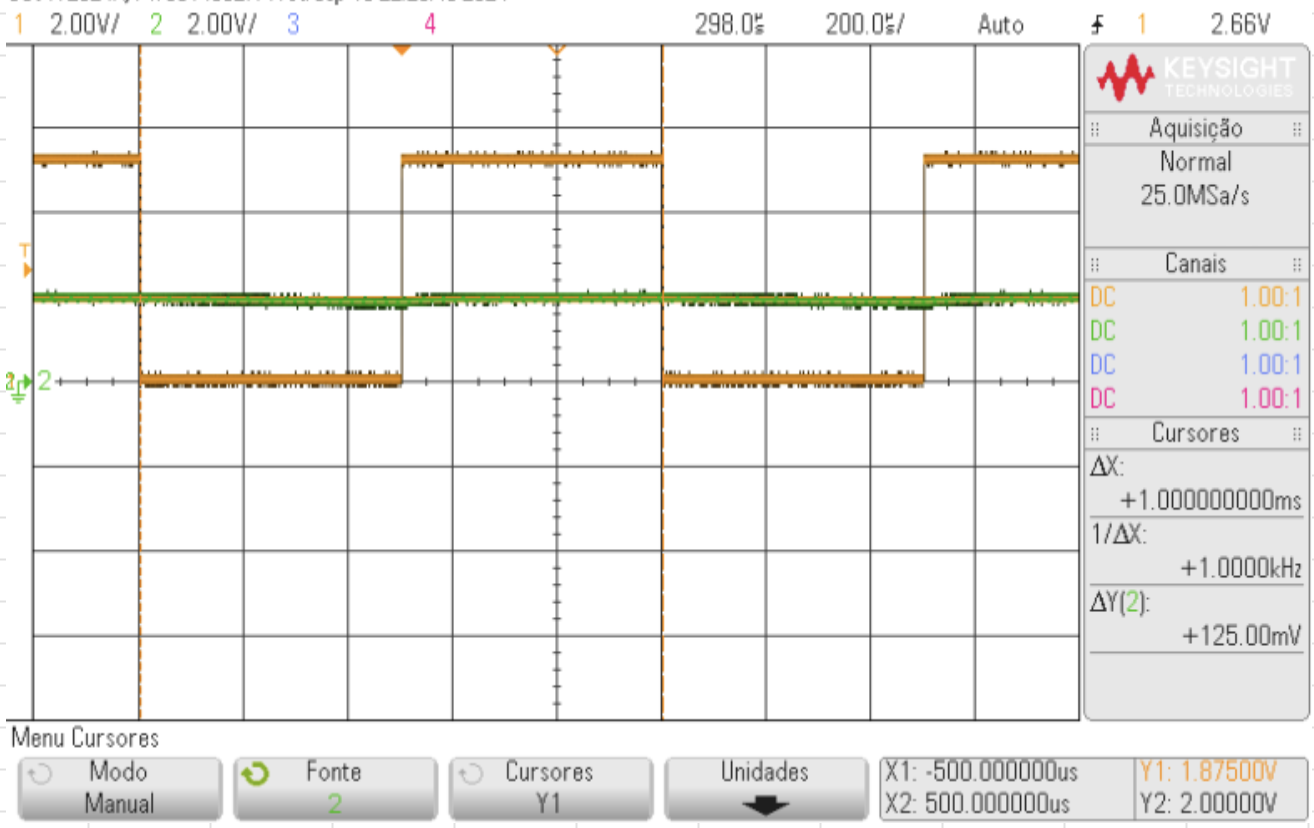
\includegraphics[width=\linewidth]{images/vdist_scope.png}
    \caption{Observed $v_{dist}$ signal from the oscilloscope. The input signal is on channel 1.}
    \label{fig:vdist}
\end{figure}

\section{LED indicator}
\subsection{Theoretical analysis}
The LED indicator in figure \ref{fig:led_indicator} consists of two main elements:
\begin{itemize}
    \item LM324 IC
    \item LEDs
\end{itemize}

The LM324 consists of four op-amps, which in this case are performing as comparators. A comparator using an op-amp compares two input voltages and outputs a high or low signal based on which input is greater. The op-amp operates in open-loop mode, meaning it amplifies the difference between the inputs without feedback, driving the output to saturation levels near the supply voltage. This makes it useful for converting an analog signal into a digital one.\\

The reference voltage is at the non-inverting input, the calculated values, using the voltage divider formula, are in table (\ref{tab:led_values}). In open-loop mode, the output of the ampop is given by $A \times (v_+ - v_{-})$, where A is the open-loop gain, a very large number (ideally close to infinity). When the voltage value at the inverting input ($v_{-}$) is smaller than the reference value ($v_+$), the op-amp saturates to \SI{12}{\volt}. When the reverse happens, the op-amp saturates to \SI{0}{\volt}.\\

When the output of the op-amp is \SI{0}{\volt} the LED turns ON, but when the output is \SI{12}{\volt} the LED remains OFF. Therefore, the expected input 

\begin{table}[h]
\centering
\caption{Theoretical and Measured LED Reference Voltages}
\label{tab:led_values}
\begin{tabular}{lccc}
\toprule
\textbf{LED} & \textbf{\makecell{Theoretical\\Voltage (V)}} & \textbf{\makecell{Measured\\Voltage (V)}} & \textbf{\makecell{Difference\\(\%)}} \\
\midrule
Green LED (A)  & 2.57 & 2.638 $\pm$ 0.005 & 2.64 \\
Yellow LED (B) & 2.06 & 2.106 $\pm$ 0.001 & 2.23 \\
Red LED (C)    & 1.54 & 1.582 $\pm$ 0.005 & 2.73 \\ 
Red LED (D)    & 1.03 & 1.052 $\pm$ 0.008 & 2.18 \\
\bottomrule
\end{tabular}
\end{table}

\begin{table}[h]
\centering
\caption{LED Combinations and Corresponding Input Voltage Ranges}
\label{tab:led_combinations}
\begin{tabular}{lc}
\toprule
\textbf{LED Combination} & \textbf{Input Voltage Range (V)} \\
\midrule
(A, B, C, D) & $v_i \geq 2.7$ \\
(B, C, D)    & $2.06 \leq v_i < 2.7$ \\
(C, D)       & $1.54 \leq v_i < 2.06$ \\
(D)          & $1.03 \leq v_i < 1.54$ \\
None         & $v_i < 1.03$ \\
\bottomrule
\label{table2}
\end{tabular}
\end{table}

The LED with the highest voltage determines the state of the other leds. If the LED A is turned ON, all LEDs will turn ON, if the LED B is turned ON, LEDs C and D are also ON, and the pattern continues until no LED is ON. Since we used resistances with 5\% tolerance, we expect experimental data to be in the range of 5\% to the theoretical predictions.

\subsection{Experimental results}

We started by measuring the reference values of the comparators (tab. \ref{tab:led_values}). There is a systematic difference of about $\approx 2.5\%$, which might indicate some systematic error. The error can be due to the components used, such as the resistors, which had a tolerance of $5\%$, and so, the error is within that margin. Another cause for this error could be that the \SI{12}{\volt} voltage source was not exact, and was slightly higher, changing all measured values to be slightly higher. The voltages for the LED combinations agree with the theoretical prevision in table \ref{tab:led_combinations}.\\

Next, we connected the output of the rectifier to the LED indicator, and drived the rectifier with filtering block with a \SI{1}{\kilo \hertz} square signal and a \SI{1}{\hertz} triangular signal to measure the input voltages each LED turned on, as we changed the amplitude of the signals:\\

\begin{table}[h]
\centering
\caption{Measured Input Voltages for Square and Triangular Waves}
\label{tab:led_measured_voltages}
\begin{tabular}{lcc}
\toprule
\textbf{LED} & \textbf{\makecell{Square Wave (\SI{1}{\kilo \hertz}) \\Voltage (V)}} & \textbf{\makecell{Triangular Wave (\SI{1}{\hertz})\\Voltage (V)}} \\
\midrule
Red LED (A)    & $3.24 \pm 0.18$ & $6.99 \pm 0.04$ \\
Red LED (B)    & $4.10 \pm 0.18$ & $9.35 \pm 0.04$ \\
Yellow LED (C) & $5.14 \pm 0.18$ & $11.68 \pm 0.04$ \\ 
Green LED (D)  & $6.25 \pm 0.18$ & $13.88 \pm 0.04$ \\
\bottomrule
\end{tabular}
\end{table}

At first, when observing the oscillating wave on the oscilloscope, we measured the amplitude by manually identifying the wave's peaks and valleys. In other words, our method lacked precision, leading to an uncertainty of \SI{0.4}{\volt} (double the \SI{0.18}{\volt} we later achieved). To improve accuracy, we began using the oscilloscope’s waveform capture feature, which displayed the complete oscillation of the wave. This allowed us to measure the amplitude more precisely using two vertical cursors, as we could now confidently locate the peak and valley positions.\\

This uncertainty was directly tied to the cursor-based measurement. While measuring the peak, every slight adjustment of the cursor resulted in a small voltage change. Once we could no longer distinguish between the peak value and $\pm \SI{0.09}{\volt}$, we defined that as our measurement uncertainty. Since the same process applied to measuring the valley, the total uncertainty doubled to \SI{0.18}{\volt}.\\

We applied a similar approach to the triangular signal. Since positioning the cursor at the peak of a triangular wave is easier than on the relatively wide plateau of a square wave, we achieved lower uncertainty when measuring the triangular signal.\\

As expected, the amplitudes are much higher (double) for the \SI{1}{\hertz} wave, as the rectifier with filtering attenuates low frequencies and lets pass the higher frequency \SI{1}{\kilo \hertz} signal. Even though the triangular signal has a higher \textit{RMS} (effective) voltage value ($A$ vs. $\frac{A}{\sqrt{3}}$), the frequency of the signal has a more sharp effect because of the high pass filtering.

\section{Bandpass filtering}
\subsection{Theoretical analysis}
The bandpass filtering block in figure \ref{fig:biquad_filter} is designed to eliminate the noise sources that may affect the integrity of the signal.
The bandpass filtering will be realised using a Raunch biquadratic (biquad) section. Biquads are second order filters (have two poles), and for a bandpass filter, the biquad formula for the transfer function is:

\begin{equation}
    T(s) = \frac{a_1 s}{s^2 + \frac{w_0}{Q}s + {w_0}^2}
\end{equation}

The parameter $Q$, usually called pole quality factor, determines the distance of the poles from the $j\omega$ axis: the higher the value of $Q$, the closer the poles are to the $j\omega$ axis, and the more selective the filter response becomes. Higher $Q$ values are harder to realise experimentaly.\\

The parameter $\omega_0$ is called the filter center frequency. At $w = w_0$ the magnitude response reaches its maximum value.\\

The transmission zeros are determined by the coefficients in the numerator. Since this is a bandpass filter, only the coefficient $a_1$ is present. This parameter scales the gain of the filter. At the center frequency the gain is given by:
\begin{equation}
    G(\omega_0) = \frac{a_1 \times Q}{\omega_0}
\end{equation}

The circuit in figure \ref{fig:biquad_filter} implements a Raunch biquad section. Capacitor $C_5$ is a \textit{bypass capacitor}, filtering any unwanted high-frequency noise from the \SI{12}{\volt} DC power source.\\

To calculate the transfer function for the filter in figure \ref{fig:biquad_filter}, we first started by applying Kirchhoff's current law to the op-amp input node and $v_{IR}$ node, solving the resulting system of equations gives the following transfer function:

\begin{equation}
    T(s) = - \frac{\frac{s}{C_3 R_8}}{s^2 + \frac{(C_3 + C_4)}{R_9 C_3 C_4} s + \frac{R_{10} + R_{8}}{C_3 C_4 R_{10} R_{8} R_{9}}}
\end{equation}

The graph of the magnitude response is represented in figure \ref{graph:magnitude_response_filter}. There is a jump from -90º to -270º at the center frequency. The phase is continuous, but at the end of the trigonometric circle (0º and -360º( there is a phase jump, which explains the "discontinuous" effect at the center frequency.
From this transfer function the relations for a biquad section are in the following equations:
\begin{align}
    a_1 &= -\frac{1}{C_3 R_8} \\
    \omega_0^2 &= \frac{R_{10} + R_{8}}{C_3 C_4 R_{10} R_{8} R_{9}} \\
    Q &= \sqrt{\frac{R_{10} + R_{8}}{C_3 C_4 R_{10} R_{8} R_{9}}} \frac{R_9 C_3 C_4}{C_3 + C_4}\\
    \label{eq:biquad_transfer_function}
\end{align}

The calculated values for each parameter are in table \ref{tab:bandpass_filter_values}.\\

To confirm our theoretical prediction of the transfer function, a simulation using LTSpice was used:

\begin{figure}
    \centering
    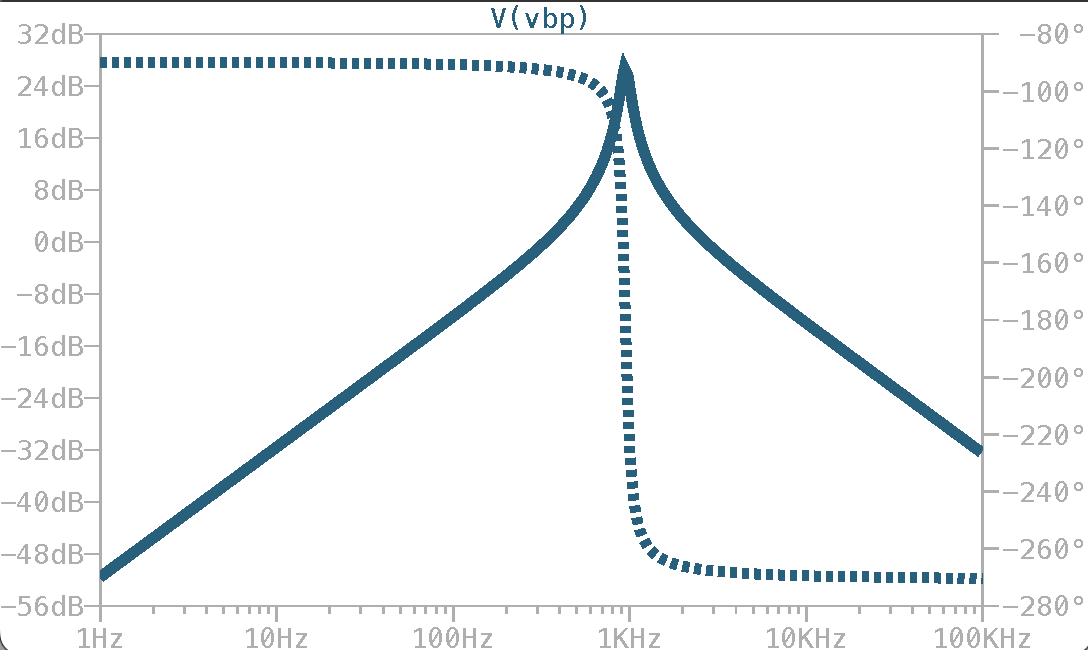
\includegraphics[width=\linewidth]{images/bandpass_transfer.png}
    \caption{Bode plot of the transfer function of the filter simulated using LTSpice.}
    \label{fig:raunchbiquad-sim}
\end{figure}

The LTSpice simulation agrees with the transfer function derived in equation \ref{eq:biquad_transfer_function} and plotted in figure \ref{graph:magnitude_response_filter}. Before reaching the center frequency, the phase difference is $-90$º and after is $-270$º. The shape of the magnitude response due to:

\begin{itemize}
    \item The zero at DC contributes to the initial gain increase of 20 db/dec
    \item The complex conjugate poles (symmetric to the center frequency) introduce a resonant peak and subsequent gain decrease if 20 db/dec.
    \item The net effect of these elements produces the characteristic bandpass response, with the asymptotic slopes explained by the frequency-dependent contributions of the numerator and denominator in the transfer function.
\end{itemize}

\subsection{Experimental results}
We first started by assembling the circuit, and to verify experimentally the transfer function derived in \ref{eq:biquad_transfer_function}, injected a low amplitude $\SI{0.30}{\volt}$ sinusoidal wave with $\SI{0.5}{\volt}$ DC component (offset). The amplitude should be small in order to not saturate positively the op-amp, there should be a continuous component in order to not saturate negatively the op-amp (the signal should never be negative). 

To estimate the location of the center frequency we started by using the theoretical prediction and looking for the phase shift between the input and output signals. When the input frequency is lower than $\omega_0$, the phase shift is $-90$º, when it is higher, the phase shift is $-270$º. The switch in phase occurs at $\omega_0$. We estimated $\omega_0$ to be around $\SI{1000}{\hertz}$.\\

We then varied the frequency from \SI{6}{\hertz} to \SI{26}{\kilo \hertz}, taking more experimental points near the center frequency. Measured the output of the filter, $V_{BP}$, and calculated the gain of the filter for each frequency, as well as the phase difference between input and output. Performing a fit using the software Gnuplot gives the experimental values in table \ref{tab:bandpass_filter_values}.

\begin{table}
\centering
\caption{Theoretical and Experimental Values for the parameters of the bandpass filter.}
\label{tab:bandpass_filter_values}
\begin{tabular}{lccc}
\toprule
\textbf{Parameter} & \textbf{\makecell{Theoretical\\Value}} & \textbf{\makecell{Experimental\\Value}} & \textbf{\makecell{Difference\\(\%)}} \\
\midrule
$a_1$        & 14872  & $16042 \pm 264$  & 7.87    \\
$Q$          & 8.83    & $7.19 \pm 0.34$   & -18.57  \\
$w_0$ (Hz)   & 946     & $1013 \pm 4$     & 7.13    \\
$G(\omega_0)$ (dB) & $26.9 \pm 1.27$ & $25.2 \pm $ & -6.32 \\
\bottomrule
\end{tabular}
\end{table}

The value of $\frac{\chi^2}{N_{df}}$ is 1.14, which indicates a good fit of the experimental data, as seen in figure \ref{graph:magnitude_response_filter}. The experimental points for the phase difference are not plotted for simplicity of visualization, but they closely match the theoretical prediction. All errors where propagated linearly. \\

There is a noticeable difference from the theoretical value of the pole quality factor, $Q$, which can be attributed, in great part, to the non exact value of the components used. Slight deviations from the theoretical values will have a big impact in the value of $Q$. The parameters $a_1$ and $\omega_0$ have both a similar difference to the expected value, which might indicate that $R_8$ and $C_3$ (values common to both parameters) have a real value smaller than their theoretical value. Considering that the resistance $R_8$ used had $5\%$ tolerance and the capacitor $C_3$ had $20\%$ tolerance (M), we can expect, at most, a difference in about $30\%$ of the value of $a_1$ and around $60\%$ on the value of $\omega_0$ and $Q$, as shown in \ref{appendix:calculations}). Considering that, to reduce the error in $Q$, a capacitor with a lower tolerance should have been used.\\

To test the influence of the frequency, amplitude and duty cycle of the square signal in the filter's output, we aqquired the output of the filter for 27 combinations of:
\begin{itemize}
    \item $\SI{100}{\hertz}$, $\SI{1000}{\hertz}$ and $\SI{10000}{\hertz}$.
    \item 25\%, 50\% and 75\% duty cycle.
    \item \SI{0.1}{\volt}, \SI{0.3}{\volt} and \SI{1}{\volt}.
\end{itemize}\\

We can conclude that:

\begin{itemize}
    \item At \SI{1}{\kilo \hertz}, near the center frequency of the bandpass filter, the signal is more prominent, with maximum amplitude, as this is where the filter is designed to operate efficiently.
    \item If the input amplitude of the rectangular signal is increased or decreased, you should expect the output amplitude of the filter to follow the same trend but only for frequencies within the passband.Outside of the passband, the output amplitude will remain low even if the input amplitude is increased.
    \item When the duty cycle differed from 50\%, a higher output amplitude was detected. The signal includes additional harmonics (due to the asymmetry), which may fall within the passband of the filter. As a result, more energy is transmitted through the filter, leading to an increase in the amplitude of the filtered signal. 
    \item The strength of the output signal of the filter is directly correlated with the LEDs that are on, as shown in LED display section.
\end{itemize}


\begin{figure}
    \centering
    \resizebox{\linewidth}{!}{
        \begin{gnuplot}[terminal=cairolatex, scale=1]
R10 = 1.2e3        # R10 = 1.2 * 10^3 ohms
R8  = 8.2e3        # R8  = 8.2 * 10^3 ohms
R9  = 330e3        # R9  = 330 * 10^3 ohms
C4  = 10e-9        # C4  = 10 * 10^-9 farads
C3  = 8.2e-9       # C3  = 8.2 * 10^-9 farads

i = sqrt(-1)

# Define the function H(x)
H(x) = -1 / ( R8 * ( (1 / (R9 * (i * 2*pi*x) * C4)) * ( (i * 2*pi*x)*(C3 + C4) + 1/R8 + 1/R10 ) + (i * 2*pi*x * C3 ) ) )

# Define the magnitude function
f(x) = 20*log10( abs( H(x) ) )

# Define the phase function in degrees, adjusted to range from -90 to -270 degrees
phi(x) = - arg( H(x) ) * (180 / pi ) - 180

# Set up the plot for magnitude and phase response
set title "Theoretical bode plot and magnitude experimental points
set xlabel "Frequency (Hz)"
set ylabel "Gain (dB)"
set y2label "Phase (degrees)"
set xrange [1:100000]
set logscale x
set grid
set key top left
set key at 20, 27 spacing 1.4 font ",3"
set samples 1000

# Configure y-tics for both left and right axes
set ytics nomirror
set y2tics
set y2range [-400:0]

# Define the data directly in the script
$Data << EOD
6     -36.27789627
20    -24.90539774
63    -15.92740937
250   -3.775266765
500   3.950716005
600   6.782034575
628   7.576905455
700   9.931351271
800   13.63218029
900   18.88142427
950   22.70516838
970   24.17265772
1000  24.96232479
1100  20.87482441
1300  13.56766947
2000  5
7000 -8
26000 -20
EOD

# Plot the theoretical response and experimental points
plot f(x) title "Magnitude" lw 2, \
     phi(x) title "Phase" with lines dashtype 2 lw 2 lc rgb "blue" axes x1y2, \
     $Data using 1:2 with points pt 2 ps 1 lc rgb "red" title "Experimental Points"
\end{gnuplot}

    }
    \caption{Bode plot of the transfer function of the Raunch biquad section, including the experimental points.}
    \label{graph:magnitude_response_filter}
\end{figure}


\section{555 Oscillator}
\subsection{Theoretical analysis}

The 555 Timer IC can be connected either in its monostable mode, thereby producing a precision timer of a fixed time duration, or in its bistable mode to produce a flip-flop type switching action. But we can also connect the 555 timer IC in an astable mode to produce a very stable 555 Oscillator circuit for generating highly accurate free running waveforms whose output frequency can be adjusted by means of an externally connected RC tank circuit consisting of just two resistors and a capacitor.\\

The 555 oscillator (fig. \ref{fig:555IRSCHEME}) operates as follows: we begin with the flip-flop inside the NE 555 oscillator in reset mode for a duration of \( T_L \). During this time, the output voltage (pin 3) is close to \SI{0}{\volt}, while the voltage applied to the transistor remains high. In this situation, the transistor is turned on, causing the capacitor to discharge through \( R_{12} \). This is the period when the trigger voltage (pin 2) decreases exponentially towards 0, following the equation below:

\begin{equation}
V_C(t) = V_{CC} \left( e^{-\frac{t}{C_7 \times R_{12}}} \right)
\label{eq:charging}
\end{equation}

The duration \( T_L \) corresponds precisely to the time it takes for the trigger voltage to reach the threshold voltage of comparator 2 (\( V_{TL} = \frac{1}{3} V_{cc} \)). When this happens, the output of this comparator goes high and sets the flip-flop, resulting in an output voltage equal to \( V_{cc} = 12V \). Once the transistor is turned off, the capacitor begins to charge through the series combination of \( R_{11} \) and \( R_{12} \), causing the voltage at pin 7 to increase (following equation \ref{eq:discharge}), along with an exponential increase in the trigger voltage (following equation \ref{eq:exponential_decrease}). This continues until trigger voltage reaches the threshold voltage of comparator 1 (\( V_{TH} = \frac{2}{3} V_{cc} \)), at which point the output of this comparator goes high and resets the flip-flop again:

\begin{equation}
V_C(t) = V_{CC} - (V_{CC} - V_{TL}) e^{-\frac{t}{C_7(R_{11} + R_{12})}}
\label{eq:exponential_decrease}
\end{equation}

Using equation \ref{eq:exponential_decrease}, we apply the voltage divider to obtain the discharge voltage at pin 7 (equation \ref{eq:discharge}), which increases from \SI{6.14}{\volt} to \SI{9.07}{\volt} during the interval \( T_H \), which is the time it takes to the trigger voltage to go from \( V_{TL} \) to \( V_{TH} \), as seen in figures \ref{fig:trigger_pin_scope} and \ref{fig:discharge_pin_scope}.

\begin{equation}
V_7(t) = V_{CC} \left[ 1 + \left( \frac{R_{12}}{R_{12} + R_{11}} - 1 \right) \frac{2}{3} e^{-\frac{t}{C_7(R_{11} + R_{12})}} \right]
\label{eq:discharge}
\end{equation}

From equations \ref{eq:exponential_decrease} and \ref{eq:charging}, we can obtain intervals \( T_H \) and  \( T_L \) (respectively), which take the following values:


\begin{equation}
T_H = C_7(R_{11} + R_{12}) \ln\left(\frac{V_{CC} - V_{TL}}{V_{CC} - V_{TH}}\right)
\end{equation}

\begin{equation}
T_L = C_7 R_{12}  \ln\left(\frac{V_{TH}}{V_{TL}}\right)
\end{equation}

Considering \( V_{TH} = \frac{2}{3}V_{CC} \) e \( V_{TL} = \frac{1}{3}V_{CC} \), we have:

\begin{equation}
T_H = C_7(R_{11} + R_{12})\ln 2 \approx 7.76 \times 10^{-4} \, \si{\second}
\end{equation}


\begin{equation}
T_L = C_7 R_{12} \ln 2 \approx 2.08 \times 10^{-4} \, \si{\second}
\end{equation}

Finally, we can calculate the period and duty cycle:

\begin{equation}
T = T_H + T_L = 9.84 \times 10^{-4} \, \si{\second}
\end{equation}

\begin{equation}
\text{Duty Cycle} = \frac{T_H}{T_H + T_L} = 78.86\%
\end{equation}

To validate the obtained results we simulated the oscillator circuit using the software LTSpice \ref{appendix:ltspice_settings}.

\subsection{Experimental results}

After assembling the circuit in the laboratory, we obtained measurements for the three pins indicated in the guide, from which we derived the three graphs in this subsection. Starting with the trigger voltage measurement, we obtained a result very similar to the simulation in LTspice \ref{fig:ltspice_sim_settings_week2}, which, as expected, aligns with what we had predicted in the theoretical part.

\begin{figure}
    \centering
    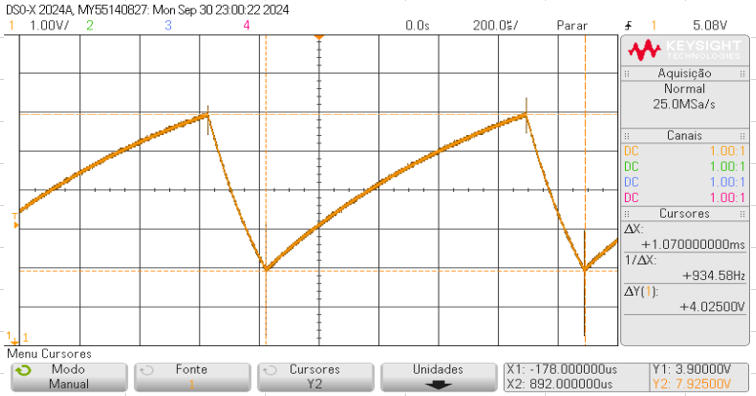
\includegraphics[width=\linewidth]{images/sinal_v2.png}
    \caption{Observed signal in the oscilloscope at pin 2 (trigger).}
    \label{fig:trigger_pin_scope}
\end{figure}

A note regarding the values we obtained for \( V_{TL} \) and \( V_{TH} \):

\begin{table}[h]
\centering
\caption{Theoretical and Experimental Values for threshold voltages.}
\label{tab:threshold_values}
\begin{tabular}{lccc}
\toprule
\textbf{Parameter} & \textbf{\makecell{Theoretical\\Value}} & \textbf{\makecell{Experimental\\Value}} & \textbf{\makecell{Difference\\(\%)}} \\

\midrule
$ V_{TL} (V)$        &  4.00  & $3.90 \pm 0.10$  & -2.50   \\
$ V_{TH} (V)$          & 8.00    & $7.93 \pm 0.10$   & -0.88  \\
\bottomrule
\end{tabular}
\end{table}

The experimental values obtained have an identical negative deviation among themselves, clearly pointing to a systematic error. Most likely, the cause of this error lies in the regulation of the \( V_{CC} \) value to 12 volts which, by varying sharply in short periods of time, slightly alters the values that are fractions of this number. Nevertheless, the difference between the deviations is due to the placement of the cursors, something that is not at all significant in our experimental analysis (which justifies the absence of measurement uncertainties).

Next, from the analysis of the oscillator's output, we can analyze how accurately we obtained the values of \( T_{TH} \), \( T_{TL} \), and consequently, the values of the period \( T \) and duty cycle:

\begin{figure}
    \centering
    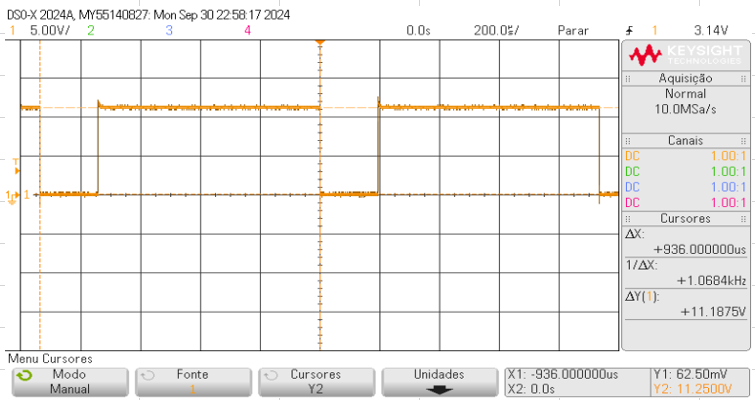
\includegraphics[width=\linewidth]{images/sinal_v3.png}
    \caption{Observed signal in the oscilloscope at pin 3 (output).}
    \label{fig:output_pin_scope}
\end{figure}

\begin{table}[h]
\centering
\caption{Theoretical and Experimental Values for intervals \( T_{H} \) and \( T_{L} \).}
\label{tab:threshold_values}
\begin{tabular}{lccc}
\toprule
\textbf{Parameter} & \textbf{\makecell{Theoretical\\Value}} & \textbf{\makecell{Experimental\\Value}} & \textbf{\makecell{Difference\\(\%)}} \\
\midrule
$ T_{L}\ (\si{\micro\second}) $        & $208$   & $195 \pm 10$   & $ -6.25$  \\
$ T_{H}\ (\si{\micro\second})$         & $776$   & $741 \pm 10$   & $ -4.51$  \\
$ T\ (\si{\micro\second})$             & $984$   & $936 \pm 14$   & $ -4.88$  \\
$ \text{Duty Cycle}\ (\%)$             & $78.86$        & $79.17 \pm 1.60$ & $ 0.39$ \\
\bottomrule
\end{tabular}
\end{table}

Regarding the obtained \( V_{CC} \) value, there is nothing more to add: the difficult regulation of this value and the placement of the cursors themselves lead to this slight difference between 11.18 V (experimental) and 12 V (theoretical).

Now, we will analyze how accurately the values obtained for the start and end of the function \ref{eq:discharge} in the interval \( T_{H} \) match what we predicted in theory, where \( V_{init} \) and \( V_{final} \) are, respectively, the initial and final values of the function in the mentioned interval.

\begin{figure}
    \centering
    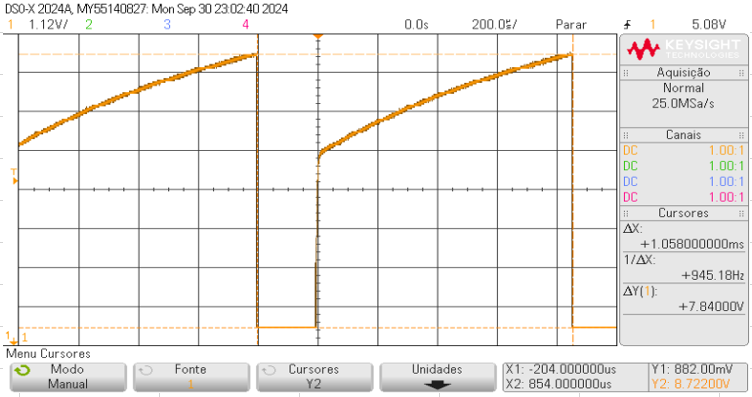
\includegraphics[width=\linewidth]{images/sinal_v7.png}
    \caption{Observed signal in the oscilloscope at pin 7 (discharge).}
    \label{fig:discharge_pin_scope}
\end{figure}

\begin{table}[h]
\centering
\caption{Theoretical and Experimental Values for discharge pin.}
\label{tab:threshold_values}
\begin{tabular}{lccc}
\toprule
\textbf{Parameter} & \textbf{\makecell{Theoretical\\Value\\(V)}} & \textbf{\makecell{Experimental\\Value\\(V)}} & \textbf{\makecell{Difference\\(\%)}} \\

\midrule
$ V_{init} $        &  6.14  &  5.92 \pm 0.10  & -3.58   \\
$ V_{final}$          & 9.07    & 8.72 \pm 0.10  & -3.86  \\
\bottomrule
\end{tabular}
\end{table}

Since their values fit within the experimental errors of our measurements, we can verify the accuracy of equation \ref{eq:discharge}, as well as its formulation in \ref{appendix:calculations}.

Finally, let's delve on the interval when the function is very close to 0. As explained, when \( T_{L} \) begins, the saturated transistor inside the oscillator causes a voltage of approximately zero volts to appear at the common node of \( R_{11} \) and \( R_{12} \). Since we can see in the figure above that cursor Y1 measures \SI{882.00}{\mili \volt}, we can, in fact, confirm that this resistance is very low (but not 0), although we were instructed to consider in the theoretical analysis a \SI{0}{\ohm} resistance for the transistor.





\section{IF Emitter and Receiver}

The circuit shown in figure \ref{fig:555IRSCHEME} has an infrared (IR) obstacle detection system. It has an IR emitter and an IR receiver that work together to detect the presence of an obstacle.\\

The SIR3333 is the IR emitter, which is essentially an infrared LED. It emits IR light when powered. The resistor labeled $R_{13}$ is placed in series with the LED to limit the current, preventing damage to the IR LED.\\

The SFH309FA component is the IR receiver, which is a phototransistor sensitive to infrared light. When the emitted IR light reflects off an obstacle, the light is then detected. In response to the detected light, the phototransistor conducts. The resistor $R_{14}$ helps convert the phototransistor’s response into a readable voltage signal.

\begin{figure}[H]
    \centering
    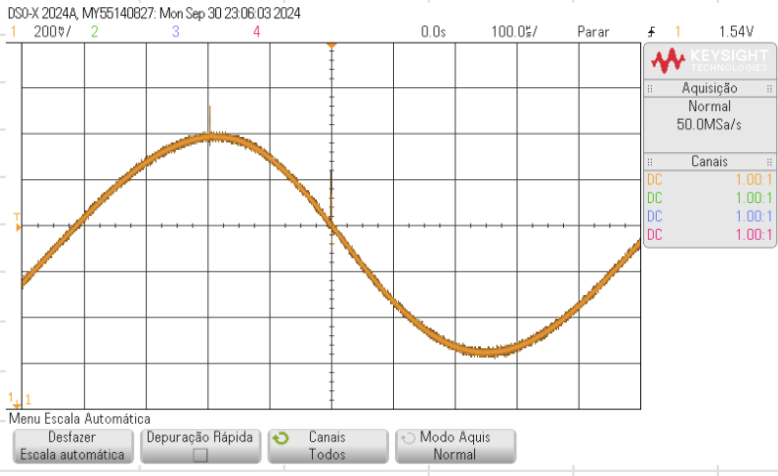
\includegraphics[width=0.9\linewidth]{images/sbiquadprox.png}
    \caption{Output of the IR receiver with the biquad \textbf{connected} and a close object.}
    \label{fig:cbiqiad}
\end{figure}

\begin{figure}[H]
    \centering
    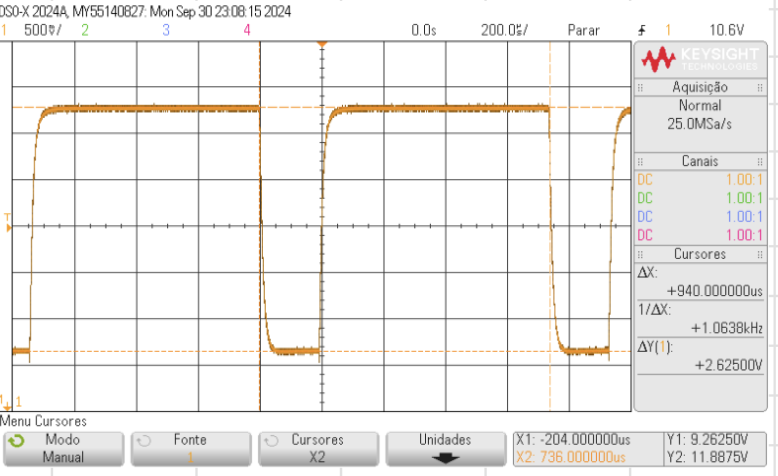
\includegraphics[width=0.9\linewidth]{images/cbiquadprox.png}
    \caption{Output of the IR receiver with the biquad \textbf{disconnected} and a close object.}
    \label{fig:sbiquad}
\end{figure}

To connect the output of the IR receiver to the biquadratic section, we had to remove resistor $R_8$ (in figure \ref{fig:biquad_filter}). Resistor $R_8$ played a major role in defining the transfer function of the filter derived in equation \ref{eq:biquad_transfer_function}, but an equivalent $R_{14}$ was placed to substitute $R_8$. If $R_8$ stayed in place, the transfer function of the filter would change.\\

As can be seen in figures \ref{fig:cbiqiad} and \ref{fig:sbiquad}, the output of the IR receiver without the biquad corresponds to part of the oscillator signal (same duty cycle, same frequency, but different amplitude and DC offset). The biquad section extracts the main frequency of the square wave and converts the square signal into a sinusoidal signal. The amplitude of the square signal is slightly higher than the amplitude of the sinusoidal wave (the biquad is applying some filtering, as the frequency of the square wave doesn't match exactly the center frequency). For an object far away, the exact same happens, but the amplitudes of the signals are lower.
 
\section{Conclusions}

In this project, we successfully designed and implemented a proximity detector using an infrared emitter and phototransistor (the full assembly can be seen in fig. \ref{fig:full_circuit}), processing the signal through rectification and filtering, and displaying the distance measurement using LEDs. When an object (we used our hands) was close to the emitter, the LEDs where all ON, as we moved our hands further away the LEDs turned OFF in sequence (REDs, Yellow and Green).\\ 

Throughout the experimentation, several challenges were encountered, providing valuable lessons for future work. Firstly, the wave generator did not display the correct peak-to-peak amplitude, necessitating the measurement of the input signal amplitude directly with the oscilloscope to ensure accuracy. Secondly, when measuring resistances, it is crucial to hold the resistor only on one end. Holding both ends can introduce a parallel resistance through the human body, affecting the measured value and leading to inaccuracies. Additionally, we observed that electrolytic capacitors have polarity and must be connected correctly to prevent malfunction or damage. Incorrect polarity can cause the capacitor to fail, sometimes explosively, as witnessed by another group. The capacitor's tolerance is a major term of error, so a lower tolerance capacitor can be used in the future to have a more precise bandpass filter. Lastly, the base used had several pins with broken wires inside, making it difficult to establish reliable connections. Moreover, the DC voltage supplied was observed to fluctuate over time, possibly due to heating effects. For future work, ensuring the integrity of the base (as well as breadboard) and monitoring the power supply stability are recommended to prevent such issues.

\subsection{Future Recommendations}

For future projects, we recommend the following:

\begin{itemize} \item Verify the functionality and calibration of all test equipment before use. \item Handle components carefully during measurements to avoid introducing unintended effects. \item Pay close attention to component specifications, such as polarity, to prevent damage. \item Use lower tolerance components (capacitor and resistor) \item Inspect and maintain the quality of the breadboard and connections to ensure reliable operation. \item Monitor power supply stability and consider using voltage regulation if necessary. \end{itemize}

These precautions will help improve the accuracy of experimental results and the overall success of the project.

\begin{thebibliography}{1}
\bibliographystyle{IEEEtran}

\bibitem{ref1}
{\it{General Electronics} classes slides}. Pedro Tomás and Gonçalo Tavares.

\bibitem{reftexas741}
{\it{UA741 OpAmp}}

\bibitem{ref2}
{\it{Microelectronic Circuits, 7th Edition}}. Sedra/Smith 2014 Oxford University Press.

\bibitem{ref3}
{\it{NE555 datasheet}}.
Texas Instruments May 1998 - Revised October 2015.

\end{thebibliography}

\clearpage
\appendices

\section{Additional Figures}
\subsection{LTSpice simulation settings}
\label{appendix:ltspice_settings}

\begin{figure}[H]
    \centering
    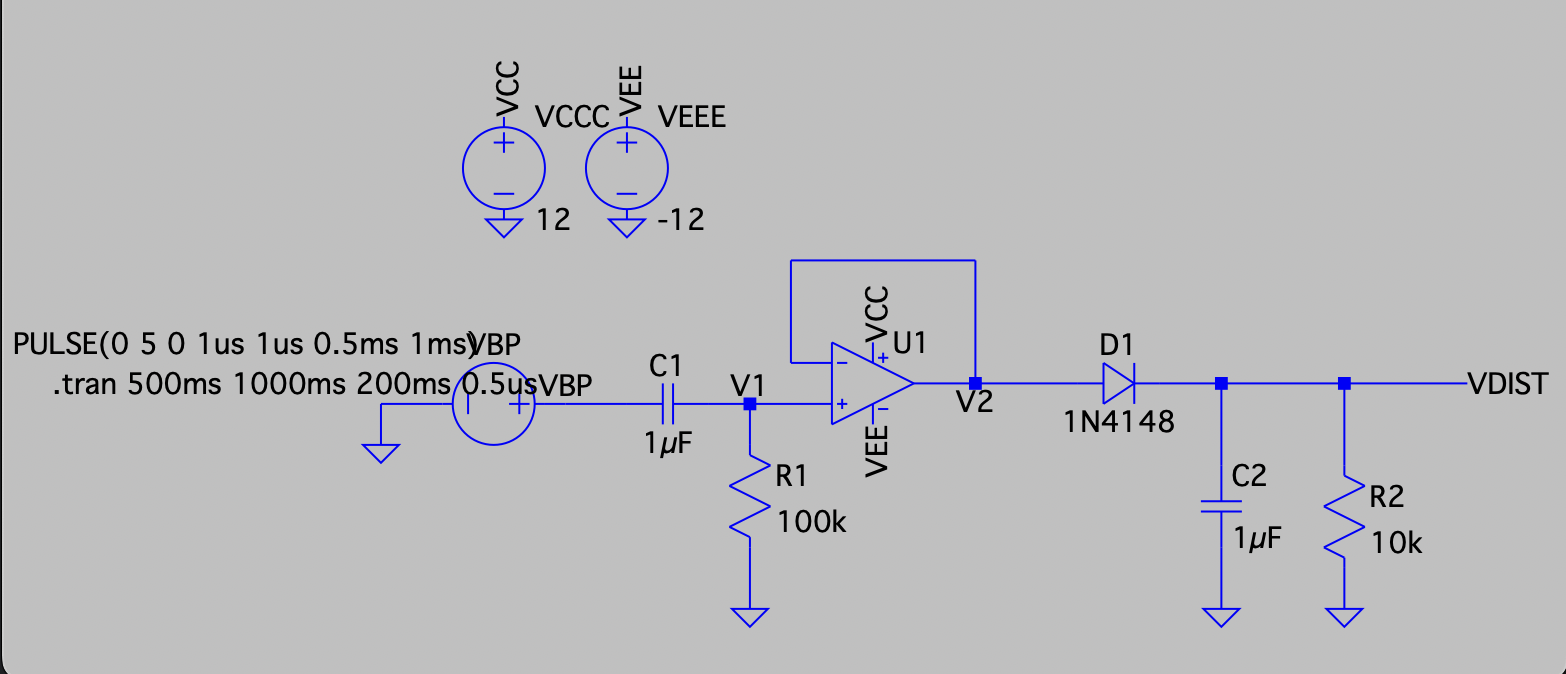
\includegraphics[width=\linewidth]{images/anexos/ltspice/week1_sim.png}
    \caption{Simulation settings for the rectifier with filtering.}
    \label{fig:ltspice_sim_settings_week1}
\end{figure}

\begin{figure}[H]
    \centering
    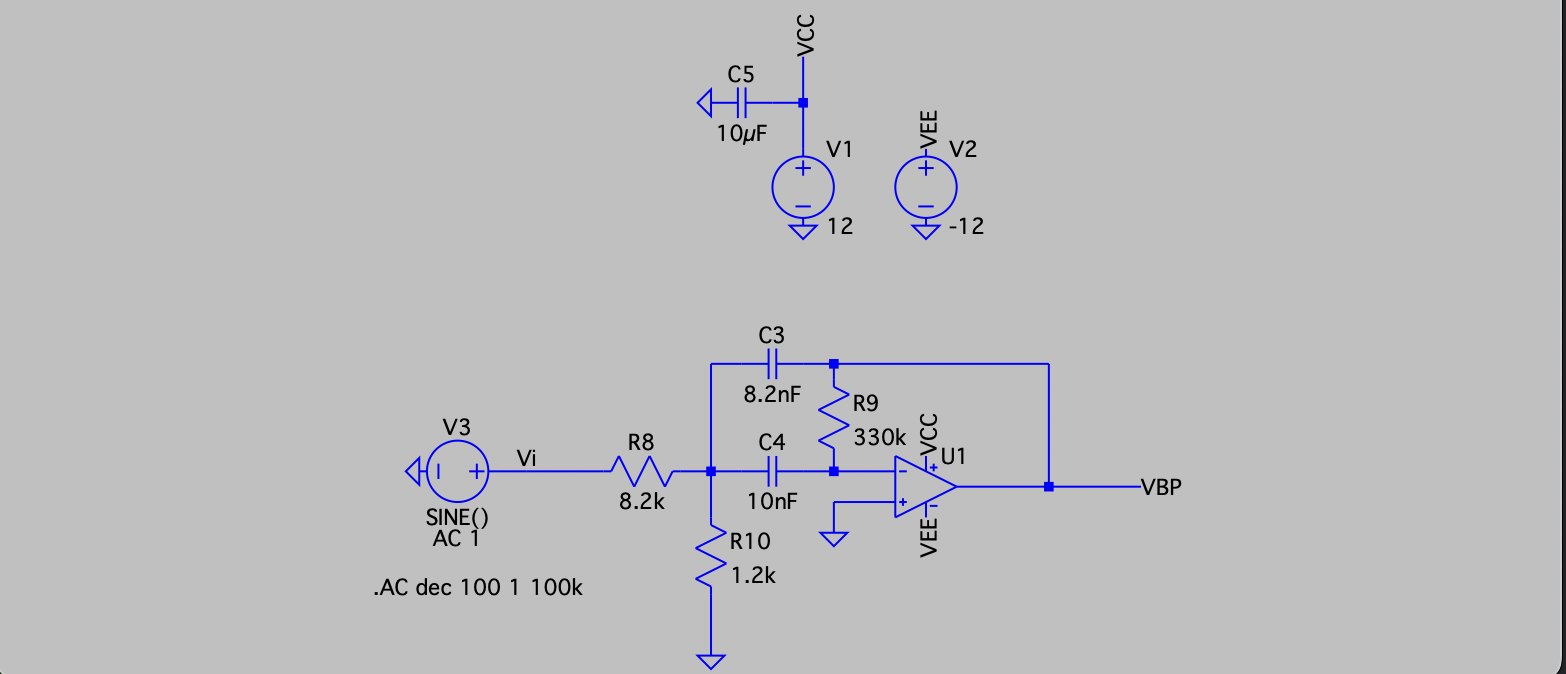
\includegraphics[width=\linewidth]{images/anexos/ltspice/week2_sim.png}
    \caption{Simulation settings for the Raunch biquadratic section.}
    \label{fig:ltspice_sim_settings_week2}
\end{figure}

\begin{figure}[H]
    \centering
    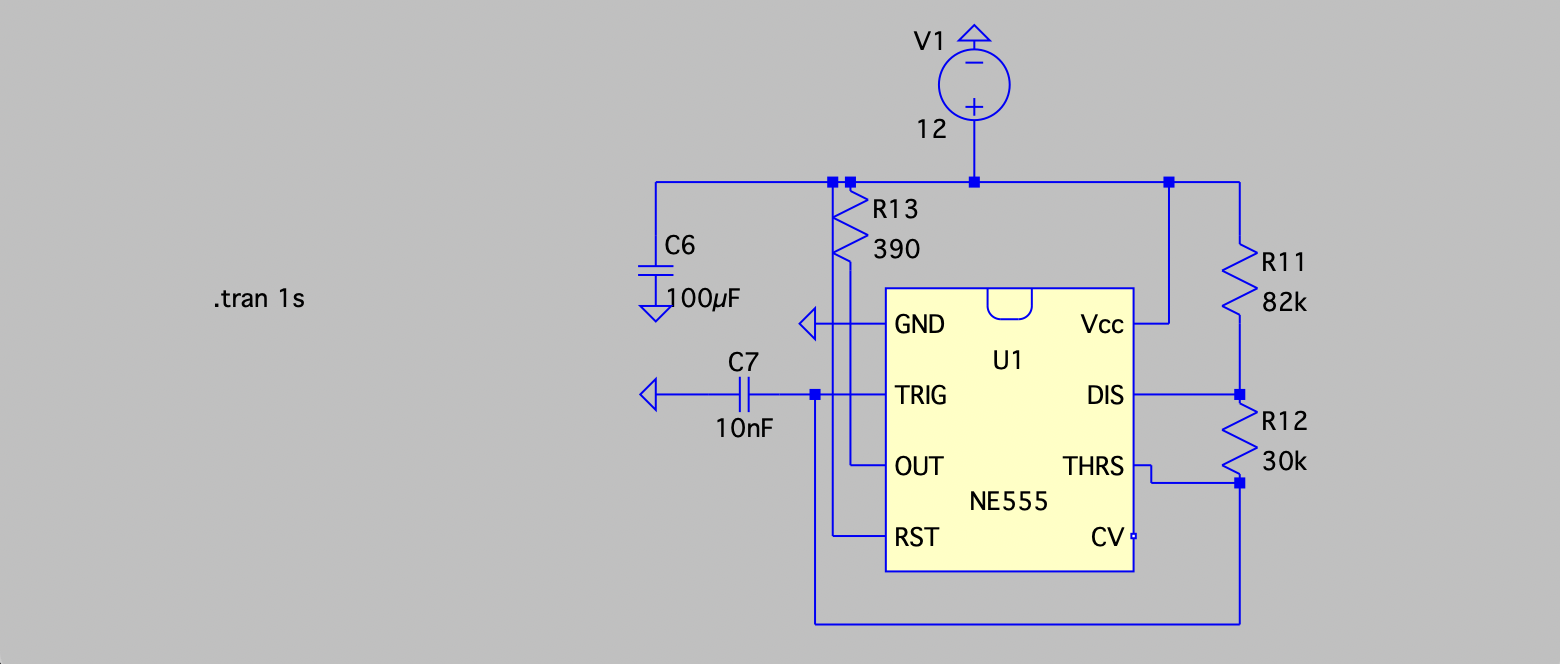
\includegraphics[width=\linewidth]{images/anexos/ltspice/week3_sim.png}
    \caption{Simulation settings for the 555 oscillator.}
    \label{fig:ltspice_sim_settings_week3}
\end{figure}

\subsection{Graphs obtained from LTSpice simulations.}

\begin{figure}[H]
    \centering
    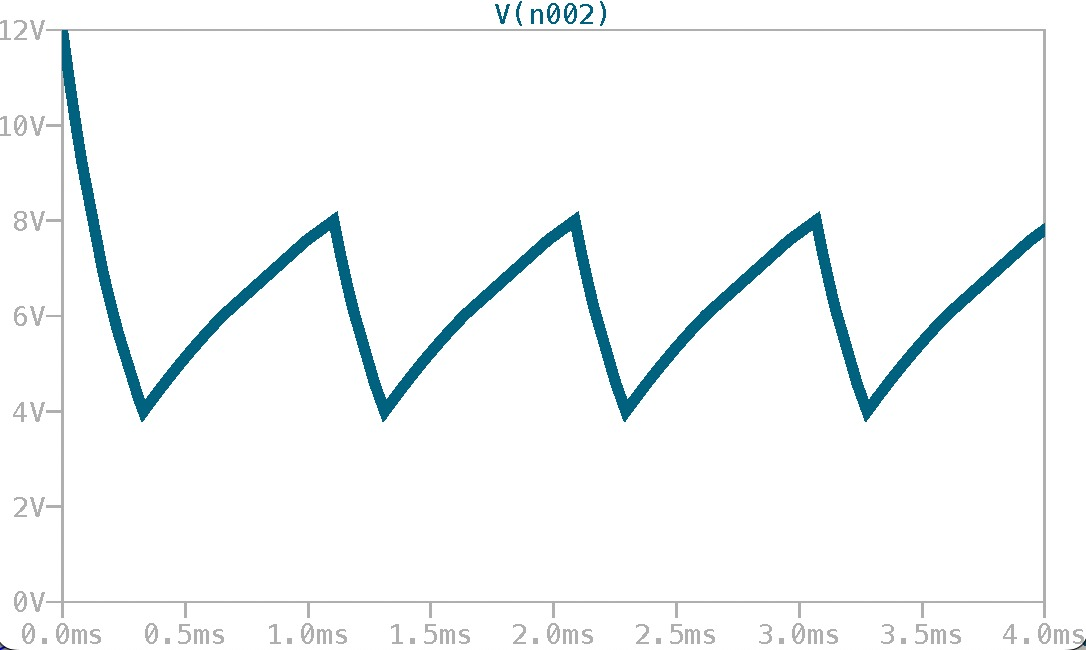
\includegraphics[width=\linewidth]{images/ltspice2.jpg}
    \caption{Graph of trigger voltage (pin 2).}
    \label{fig:ltspice_sim_settings_week2}
\end{figure}

\begin{figure}[H]
    \centering
    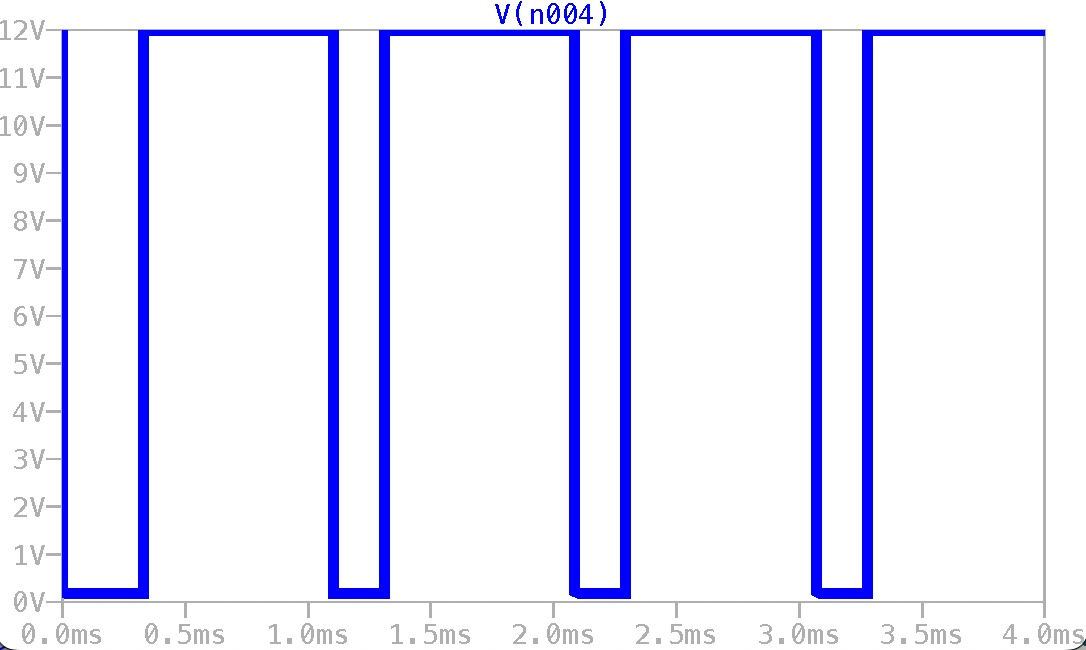
\includegraphics[width=\linewidth]{images/ltspice3.jpg}
    \caption{Graph of output voltage (pin 3).}
    \label{fig:ltspice_sim_settings_week2}
\end{figure}

\begin{figure}[H]
    \centering
    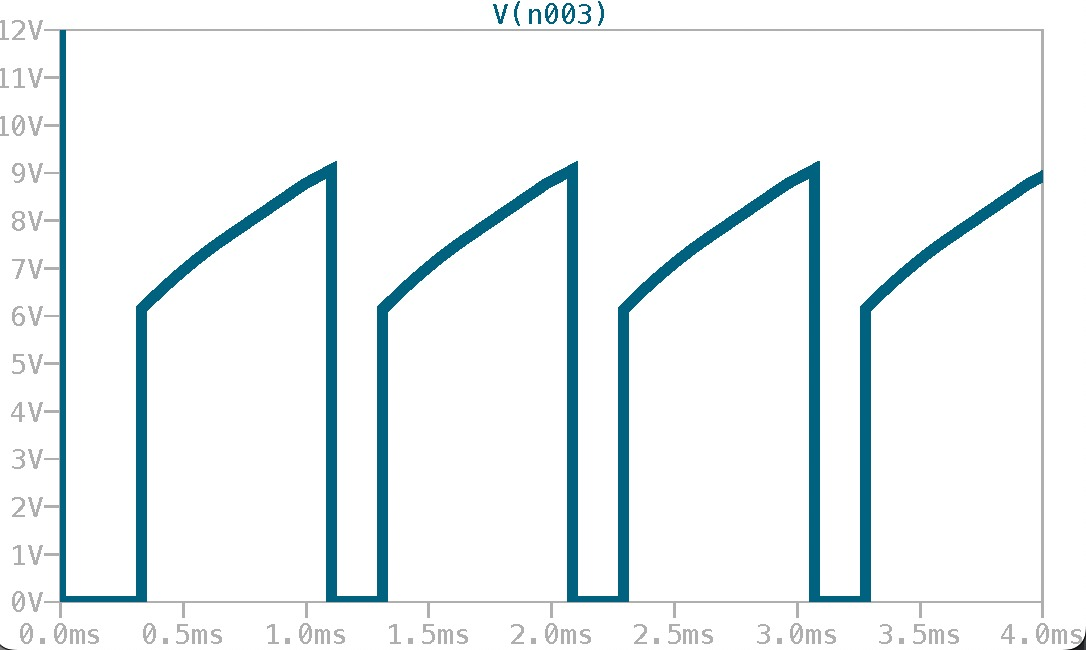
\includegraphics[width=\linewidth]{images/ltspice7.jpg}
    \caption{Graph of discharge voltage (pin 7).}
    \label{fig:ltspice_sim_settings_week2}
\end{figure}

\subsection{Circuit schematics}
\begin{figure}[H]
    \centering
    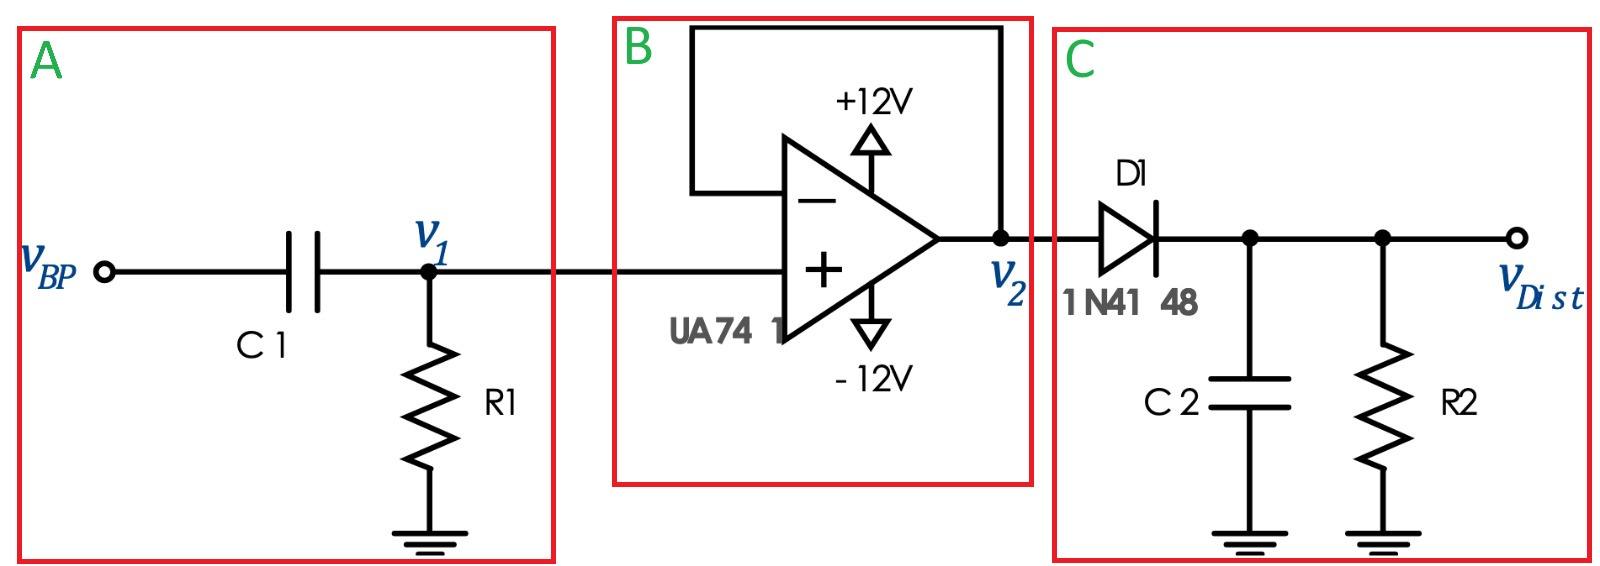
\includegraphics[width=0.9\linewidth]{images/week1_circuit_components.jpeg}
    \caption{Circuit schematic highlighting the three main components. $R_1 = \SI{100}{\kilo \ohm}$, $C_2 = \SI{1}{\micro \farad}$, $R_2 = \SI{10}{\kilo \ohm}$.}
    \label{fig:circuit_components}
\end{figure}

\begin{figure}[H]
    \centering
    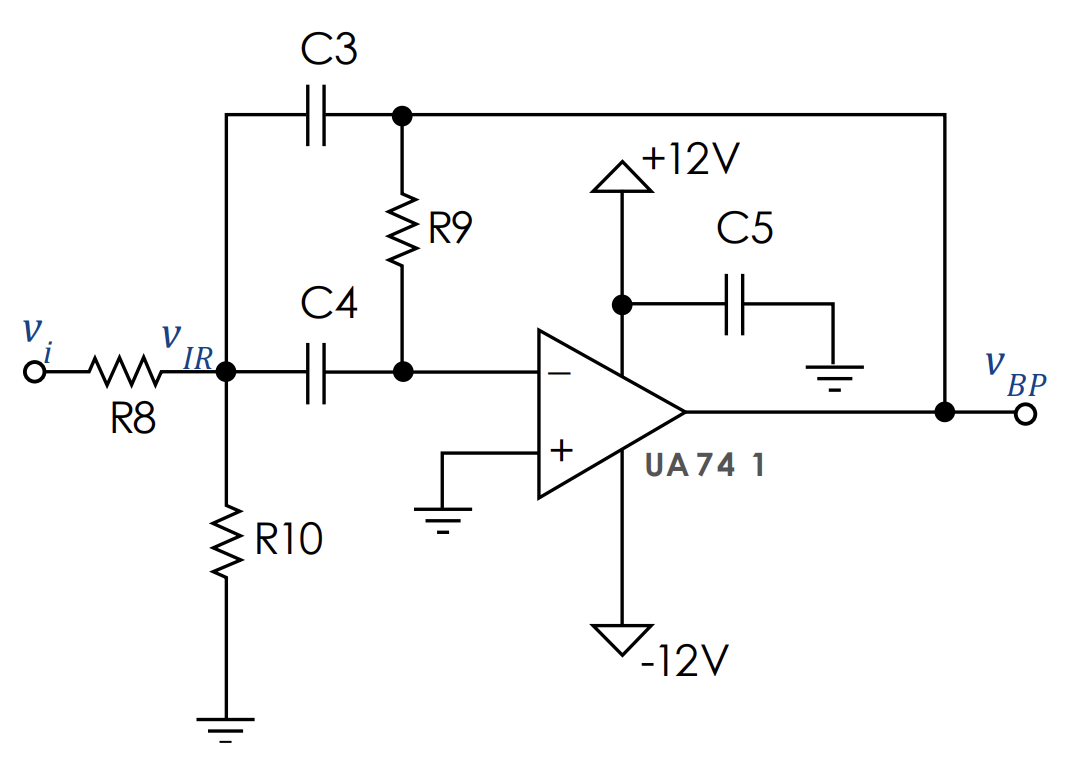
\includegraphics[width=0.7\linewidth]{images/biquad_bandpass.png}
    \caption{Circuit schematic of the Raunch biquadratic section. $R_8 = \SI{8.2}{\kilo \ohm}$, $R_9 = \SI{330}{\kilo \ohm}$, $R_{10} = \SI{1.2}{\kilo \ohm}$, $C_3 = \SI{8.2}{\nano \farad}$, $C_4 = \SI{10}{\nano \farad}$, $C_5 = \SI{10}{\micro \farad}$.}
    \label{fig:biquad_filter}
\end{figure}

\begin{figure}[H]
    \centering
    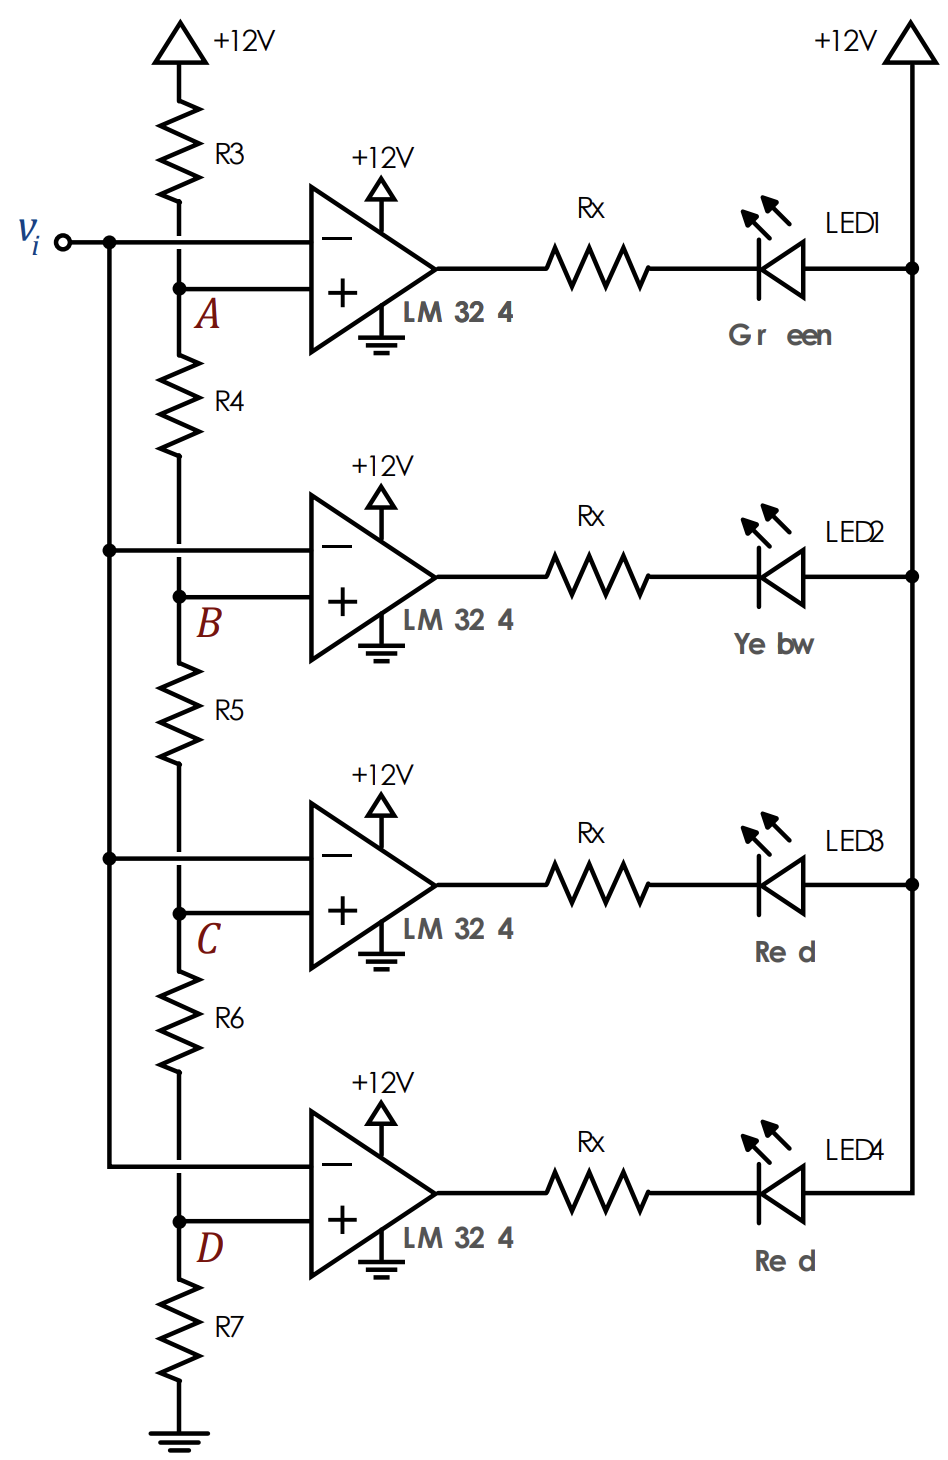
\includegraphics[width=\linewidth]{images/led_indicator.png}
    \caption{Circuit schematic of the LED indicator. $R_3 = \SI{3.3}{\kilo \ohm}$, $R_4 = R_5 = R_6 = \SI{180}{\ohm}$, $R_7 = \SI{360}{\ohm}$, $R_x = \SI{1}{\kilo \ohm}$}
    \label{fig:led_indicator}
\end{figure}

\begin{figure}[H]
    \centering
    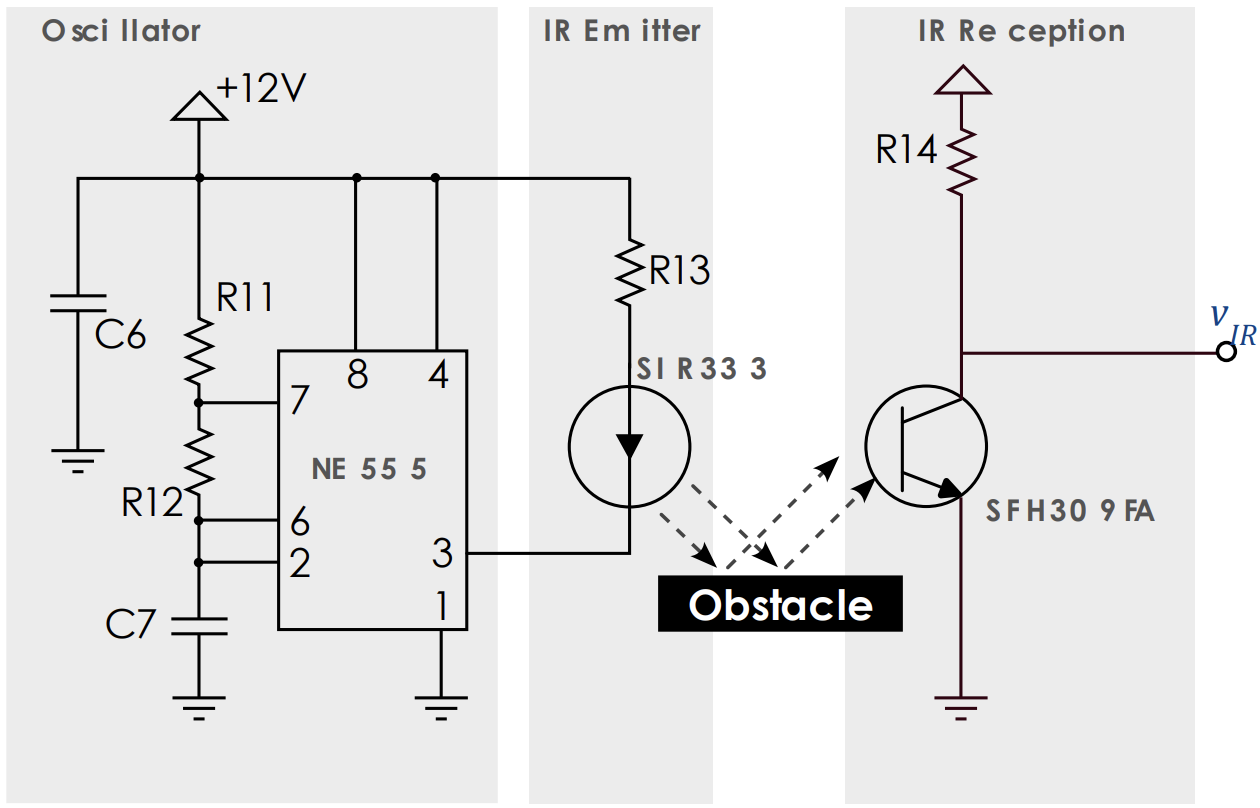
\includegraphics[width=\linewidth]{images/OSCILLATOR_DIAGRAM.png}
    \caption{Circuit schematic of the 555 oscillator and IR receiver/emitter blocks. $R_{11} = \SI{82}{\kilo \ohm}$, $R_{12} = \SI{30}{\kilo \ohm}$, $R_{13} = \SI{390}{\ohm}$, $R_{14} = \SI{8.2}{\kilo \ohm}$, $C_6 = \SI{100}{\micro \farad}$, $C_7 = \SI{10}{\nano \farad}$}
    \label{fig:555IRSCHEME}
\end{figure}



\subsection{Circuit photos}

\begin{figure}[H]
    \centering
    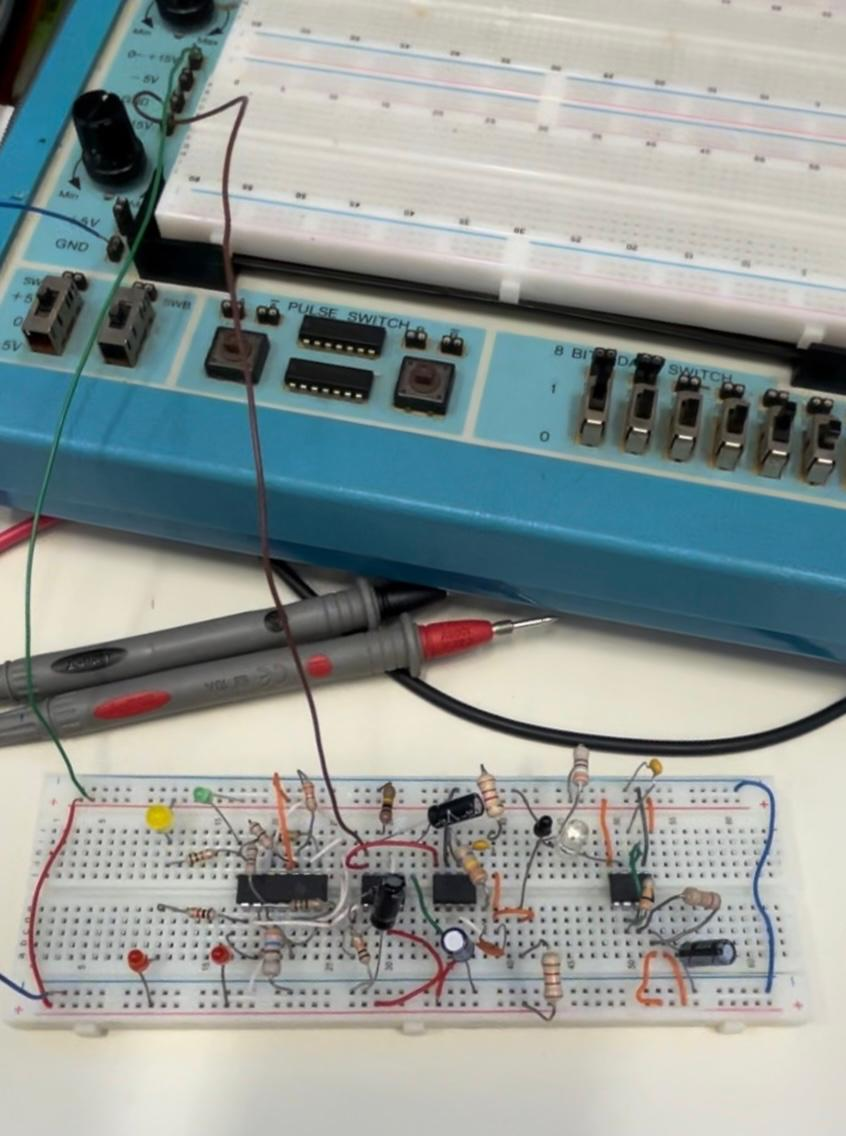
\includegraphics[width=0.7\linewidth]{images/full_circuit.jpeg}
    \caption{Picture of the full circuit.}
    \label{fig:full_circuit}
\end{figure}

\section{Detailed Calculations}
\label{appendix:calculations}
\subsection{Calculating the maximum error of the parameters $a_1$, $Q$ and $\omega_0$}
Considering only variations in the value of $C_3$ and $R_8$, for a tolerance of $20\%$ and $5\%$ respectively, the error can be calculated by:

\begin{equation}
    \delta a_1 = 1 - \frac{1}{(1 - 0.05)(1 - 0.20)} \approx 30\% \nonumber
\end{equation}

\begin{equation}
    \delta Q = \sqrt{1 - \frac{1}{(1 - 0.05)(1 - 0.20)}} \approx 60\ \nonumber
\end{equation}

$\delta \omega_0$ should have a value close to $\delta Q$.

\subsection{Calculations to get to \ref{eq:discharge}}

Start by using the voltage divider formula to calculate the potencial at pin 7:
\begin{equation}
    v_7(t) = v_c(t) + \frac{R_{12}}{R_{11} + R_{12}} \left( V_{CC} - v_c(t) \right) \nonumber 
\end{equation}

Replace $v_c(t)$ by 
\begin{equation}
   V_{CC} - (V_{CC} - V_{TL}) e^{-\frac{t}{C_7(R_{11} + R_{12})}} \nonumber
\end{equation}

Solve for $v_7(t)$ and arrive at the desired expression.


\end{document}


